%\chapter{Reasoning Models}
\chapter{Multi-step Reasoning in LLMs}\label{chap:reasoning}


\begin{learningbox}
In this chapter you will learn how  language models can solve more complex problems through {\em multi-step reasoning}. 
Specifically, you will be able to:
\begin{itemize}[leftmargin=*, nosep]
    \item Describe the {\em chain of thought} concept: how we can use in-context learning to guide the LLM to take intermediate steps in answering a query, and thus provide better answers to more complex queries.
    \item Describe how reasoning methods have increased the {\em power} of LLMs greatly, and why this power is essential for agentic LLMs to act realistically in the real world. 
    \item Write your first {\em agentic harness}: a small algorithm that calls the LLM with different prompts.  The agent harness manages the prompts and the replies from the LLM.   
    \item Explain {\em self-reflection}:  LLMs can be called in different roles by the harness, for example, to {\em evaluate} an answer, or to {\em generate} subproblems. The LLM is reflecting to improve its own answers. 
    \item Understand the role that is played by {\em memory}: how the  harness keeps track of the state of the agent, and how this state is used by the harness to manages the prompts.
    %\item Understand how an agentic harness can be used to create {\em in-context reinforcement learning}: the agent's answers improve as the LLM prompt contains more state-action-reward information. 
    \item Use the concept of {\em reinforcement learning with verifiable rewards}: where inference-time reasoning results are used for finetuning.
\end{itemize}
\end{learningbox}

\begin{comment}
    
LLMs are  good at solving language tasks, but, originally, they failed at simple multi-step reasoning tasks. For agents to take actions in the real world, they must be able to reason, in addition to being able to communicate in natural language.  In this chapter we will discuss some of the techniques that were developed for multi-step reasoning problems, in Section~\ref{sec:reasoning}. %using an in-context learning approach (future chapters will look at other learning methods---pretraining, finetuning, and metalearning). 
We will discuss the chain of thought prompting technique, show how it can be used to solve multi-step reasoning problems, and, in Section~\ref{sec:state}, we will see how its performance can be further improved using other test-time compute methods. For example, we will  discuss  techniques such as self-reflection. Some of the topics in this chapter have appeared earlier in \citet{plaat2024reasoning}.

%This chapter will focus on in-context learning. We will discuss both (regular, supervised) in-context learning and in-context reinforcement learning. The first Section will focus on methods to improve LLM  reasoning. Next, we will discuss memory and self-reflection. 


\end{comment}

\section{In-Context Reasoning}\label{sec:reasoning}
As we noted Chapter~\ref{chap:pipeline}, in large models, beyond hundreds of billions of parameters, a new kind of learning has emerged in LLMs. It is called {\em in-context learning} (ICL) or  {\em prompt-learning} \citep{brown2020language}. It is an important learning method, which we will discuss in more detail in this section. 
Then, we will discuss common benchmarks, and the chain of thought method for multi-step reasoning.


\begin{comment}
Intro
- inference time prompt with examples (1)
- Large model emerges, works because of previous knowledge (2)
- no parameter update: learning, no training (3)
What is it? 
- all data in the context window (4)
- prompt example (5)
Consequence
- few shot learning (6)
- big impact: holy grail of ML (7)
- applications: prompt engineering, reasoning (8)
\end{comment}

\subsection{In-Context Learning}
% 1 inference
In-context learning \citep{dong2022survey} occurs not at training time, but at inference time, from examples that are provided in the LLM prompt, when the model is used to answer questions. 
%2 prev knowledge emerges
These examples cause the decoder model to access relevant knowledge stored in the LLM. Because of this rich knowledge, in-context learning finds accurate results with few examples, which is why it is a so-called {\em few-shot} learning method. %ICL is learning from these few examples in the prompt, in combination with the knowledge already present in the model. 
The few-shot learning is made possible by the large size of the model, containing  rich and varied knowledge on many topics.
%, enables this %this new type of 
%few-shot learning at inference time. 

\paragraph{Learning, not Training}
%3 no para update
A main difference between in-context learning and finetuning or pretraining is that in-context learning does not change the  parameters of the transformer.
Since no model-parameters are changed at inference time, it is not a {\em parameter training} method; however, since it does learn an answer from provided examples, it is a {\em learning} method. 
%
%
%Pretraining includes forward and backpropagation phases where the parameters are changed, in-context learning consists of a single forward pass through the model.\footnote{In a forward pass the model calculates $f_\theta(x) \rightarrow \hat{y}$  the estimate $\hat{y}$ of the target for a single input example $x$, in the backward pass the model parameters $\theta$ are adjusted by backpropagation from a loss function such as $(\hat{y}-y)^2$.} 
%Such (cheap) few-shot ICL works because of the rich knowledge that has been encoded in the LLM in the (expensive) pretraining and finetuning phases.  
%Prompt-learning is based on the powerful generalization potential of LLMs.
%The models are able to perform few-shot or even zero-shot
%learning, using their knowledge on many different topics to
%adapt to scenarios without the need for the prompt to provide more
%than few or no labeled data.
%4 all data in context
A consequence is that ICL has the disadvantage of forgetfulness: since model parameters remain unchanged, all learned information is lost between LLM calls. To share information between LLM calls, previous results must be added to the prompt of the next call, in the context window, as extra learning examples. 

\paragraph{Context Window}
How does in-context learning work?
%4 context window
The part of an LLM in which the prompt is written is  called its {\em context window}.  The decoder model learns inside this context window, from the examples that are provided in the prompt. 
%4 context window size
A point to note is that  all examples that the answer is learned from must be provided together in the context window---they should fit in the prompt. Typically, the size of the context window is limited to a few thousand tokens, and only few examples can be provided: all ICL is able to perform is  few-shot learning.
%Whereas pretraining and finetuning often use datasets with many examples, and have to make many passes through the model to slowly change the many parameters, which costs much energy, ICL has the advantage of efficiency of a single forward pass. (The expensive knowledge encoding has been performed in the pretraining and finetuning phases.) 
This becomes problematic when the amount of information that we wish to learn from grows, since the context window is typically limited in size.  We might say that in-context learning suffers from long-term memory loss.

\paragraph{Example}
%5 prompt example
In in-context learning, a prompt, consisting of a few pieces of
demonstration context, is concatenated with a query question, which is given
to the context window of the language model \citep{liu2023pre}. The model will then  generate the answer  by performing a forward pass through the model. For example,
when the task is emotion recognition in a social media post, {\em I
missed the bus today}, can be followed by {\em I felt so [\_\_\_]}, and the model could answer with {\em bad}.
%
Alternatively, for translation, we could follow {\em I missed the bus today}, by
{\em French: [\_\_\_]} to request a translation.
The prompt contains background information that is recognized by the
model, selecting the desired model context. 

\paragraph{Few-shot Learning and the Holy Grail of Machine Learning}
%6 few-shot learning
In-context learning works when language models contain enough 
knowledge, allowing them to generalize on the (few) examples provided in the prompt. The user provides a few relevant examples in the prompt, in order to prime the LLM to select the right background knowledge for answering the prompted instruction.
%The prompt conditions the model. 
%
Contexts that contain a few examples
are said to perform few-shot learning. Contexts that contain
only instructions, with zero examples, are said to perform zero-shot learning. 

%7 few-shot/excite
ICL is a form of few-shot learning that caused much excitement among researchers. 
%7 many-shot/holy grail
%To understand why, we will compare it with traditional machine learning. 
In traditional machine learning, a model $f$ is trained on  dataset.
%by adjusting the parameters $\theta$ of the model $f_\theta$ in a backward pass,
%(in deep learning: by backpropagation), 
%so that a subsequent forward pass will compute a more accurate estimate $\hat{y}=f_\theta(x)$ of the target $y$. %In LLM training, the training occurs in the pretraining and finetuning  phases. %, by self-supervised methods such as masked next-word prediction, and in the finetuning phase by supervised learning. 
To achieve high accuracy on complex problems, the datasets must contain many examples. Traditional  machine learning is a form of {\em many-shot learning}, requiring many (expensive) training epochs to train the parameters of the model.
In-context learning, on the other hand, is cheap, requiring just a few examples followed by a single forward pass through the decoder model (since the expensive training has been done in the pretraining phase). Few-shot learning is something of the holy grail of machine learning:  a model that generalizes, cheaply. 




\paragraph{Practical Considerations and Prompt Engineering}
%8 cloud
In-context learning further  has the practical advantage of convenience: we can perform ICL on an LLM that runs commercially in the cloud, from our smartphone, without going through the difficulty of finding a computer to train a large model on. 


%8 prompt engineering
Although  prompts provide a user-friendly interface to LLMs, the success of in-context learning tends to be quite sensitive to the way a prompt is formulated or when different  examples are provided. Prompt-learning is brittle, and a
new field called {\em prompt engineering} has emerged to 
help human users to learn how to
make LLMs do what we want them to do \citep{radford2019language,wei2022emergent,giray2023prompt,sahoo2024systematic}.


%X system prompt/memory. move to where?
In most LLMs the context window is  provided with hidden prompts, the system prompts, to specify a particular role for the model,  to prevent the use of swear words, and, in chatbots, to have a short history of previous search results, to allow for more naturally flowing conversations. 

In-context learning has spawned much further research. One of the areas is multi-step reasoning, which is the topic of this chapter. Reasoning used to be an area where LLMs performed poorly. For example, LLMs failed at simple math exercises. To better understand this application domain we will introduce a few reasoning benchmarks. Then we will discuss an in-context learning method that greatly improved the performance of  reasoning by LLMs.

\subsection{Multi-step Reasoning Benchmarks}\label{sec:benchmarks}
Progress in artificial intelligence is measured by benchmarks. 
The research on multi-step reasoning with LLMs started with easy 
(grade school)
math word problems. Specifically  for the study of such easy reasoning the GSM8K benchmark  was composed \citep{cobbe2021training}.
GSM8K was created   with the aim of providing high quality problems, of high
diversity and moderate difficulty,  in natural language. It consists of 8500 human-written math
problems and solutions. Language models struggled to achieve good performance on this dataset before chain of thought was introduced (see the %we will explain how Chain of Thought works in  
next section).
%The performance of large language models is notably weak. 
Here is an example of a typical math word problem: 
\begin{quotation}
 \noindent  {\em Problem:} Romeo bakes 4 trays with 
%\tb{it must be "4 times two" here, I think.}
two dozen batches of cookies in a week. If these cookies are shared amongst 16 people equally, how many cookies does
each person consume?\\ 
{\em Answer:} $4\times 2\times 12/16=6$. 
\end{quotation}

The GSM8K benchmark, although it may look easy to us, turned out to be difficult for LLMs. When it was introduced, the state of the art  LLM GPT-3-175B achieved a rather low accuracy of around 15\% \citep{wei2022chain}.
%column in Table~\ref{tab:mwpbench}). 
Other  benchmarks of similar math word problems are the SVAMP varying structures benchmark \citep{patel2021nlp}, the
ASDiv dataset of diverse math problems \citep{miao2021diverse}, the AQuA dataset of algebraic
word problems \citep{ling2017program}, and the MAWPS benchmark
\citep{koncel2016mawps}. 

Later, benchmarks for other tasks were introduced, to assess LLM reasoning abilities 
in other fields of reasoning. For example, benchmarks have been developed on advanced mathematical questions (AIME \citep{codeforcesamerican}),
computer code comprehension (Spider \citep{yu2018spider}, transcoding (translating a program in one computer language to another) \citep{roziere2020unsupervised}), robotic movement (Alfworld \citep{shridhar2020alfworld}, kitchen tasks \citep{ahn2022can}), puzzle solving (Game24 \citep{yao2024tree}), creative writing \citep{yao2024tree}), board games (Checkmate problems \citep{yang2024buffer}, MineCraft \citep{fan2022minedojo}), and webpage navigation (WebShop \citep{yao2022webshop}). 
Further relevant benchmark studies also focus on games and planning problems 
\citep{ruoss2024lmact,paglieri2024balrog,wen2025thinkpatterns}. 

The goal of benchmarks is to be able to clearly compare the performance of different approaches. However,  it can be difficult to directly compare different benchmarking results, since there may be differences in the way the experiments were conducted. See \citet{kamoi2024can,shojaee2025illusion} for  a critical discussion of challenges in benchmarking LLM reasoning. 




\subsection{Chain of Thought Prompting}
Around 2022, regular LLMs of the time performed poorly on simple math word problems. Interestingly, the standard Chapter~\ref{chap:scaling} approach to improve performance of LLMs by scaling up the
size of the LLM, did not solve the problem~\citep{rae2021scaling}. The problem appeared to be somehow fundamental in nature, and researchers went looking for a different approach.
 
The LLM architecture is
a transformer-based decoder. Given a certain input, it is designed to produce a single token. LLMs are next-token predictors. When we
prompt such a decoder to  produce an answer, it does as it is instructed to: it provides an answer quickly---any answer. But that is not how humans work towards an answer in a mathematical reasoning problem, we divide the question into a sequence of steps to solve ($4\times 2\times 12/16=6$). Thus, for the LLM, what we should do instead is to prompt it to follow a well-chosen sequence of intermediate steps, answer those, and thus work towards the final answer, just as a student is taught to break down a complex problem into smaller steps, and to also provide the reasoning steps when answering a problem in school---{\em Don't just tell me the answer, but tell me how you {\em arrived} at the answer}.  Children are taught in school to break down a big problem into  a sequence of small steps, when solving a mathematical problem. Similarly, we
should guide the language model to explicitly produce such intermediate steps, and then to combine the  results.  The LLM should then  provide an answer that includes the intermediate steps, arriving at a correct result.

Thus, our few-shot prompt should contain examples of intermediate reasoning steps, instead of only examples of the final answer.
%
%
This question was studied by \citet{wei2022chain}, amongst others, who introduced the {\em chain of thought} approach. Figure~\ref{fig:cot} illustrates how the approach works, in addition to related approaches, that it  inspired.

The way to instruct an LLM to generate intermediate steps  is to manually write a prompt consisting of specific reasoning steps to answer the task (for example, calculate how many balls are in the container, or in how many pieces the pie was cut).
Indeed, when \citet{wei2022chain} tried this approach, and the LLM was prompted to rephrase information from the question as
intermediate reasoning steps in its answer, the LLM performed
much better than when it was prompted to produce a single answer. % , without reproducing  information from the question in its answer in multiple steps. 
The example from the chain of thought paper is shown in Figure~\ref{fig:cot}. When shown the longer example prompt,
      the LLM follows the longer example when answering the question  (Few-Shot CoT).  On GSM8K, the chain of thought approach  showed a large increase in  accuracy, from 16\% to 47\%. 

\begin{figure}
  \begin{center}
    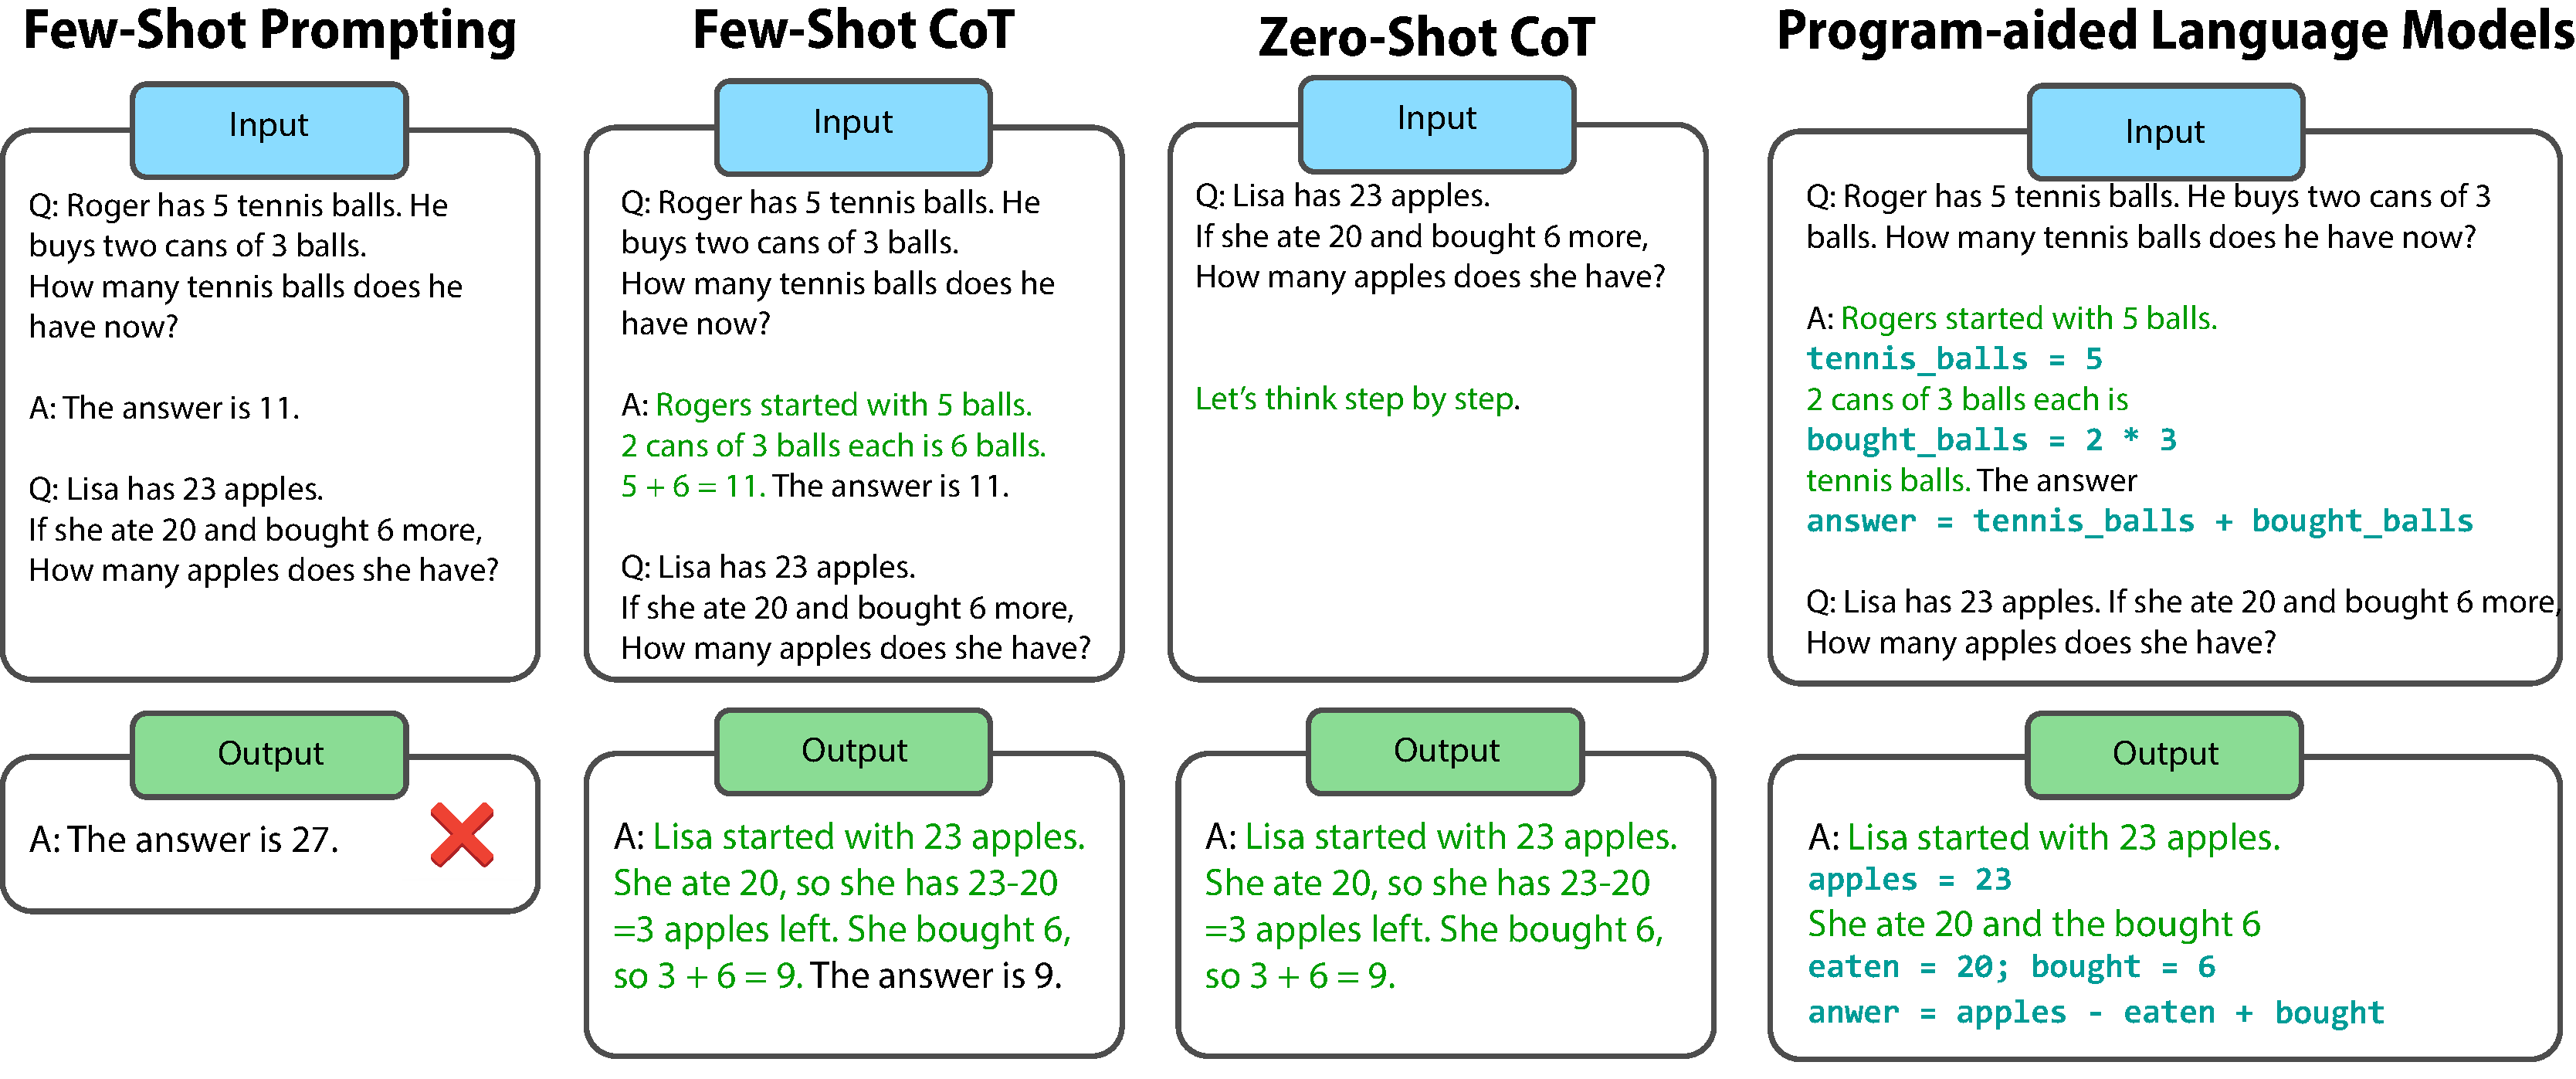
\includegraphics[width=\textwidth]{figures/cot2.pdf}
    \caption{Different Chain of Though (CoT) prompting techniques \citep{wei2022chain,kojima2022large,gao2023pal,plaat2024reasoning}. At the top the prompts, at the bottom the answers.}\label{fig:cot} \label{fig:zero} \label{fig:pal} 
  \end{center}
\end{figure}


The idea that, when prompted,  an LLM can be made to follow step-by-step instructions, has caused much excitement and has opened up further research on multi-step reasoning with LLMs. Chain of thought (CoT) has become a standard prompting approach in  LLMs since.

In the
original  paper  the prompts were hand-written by
the researchers for the individual types of problems. 
\citet{kojima2022large} go a step further.
They show that the  addition of a single task-independent sentence  ({\em Let's think step by step}) also
significantly improves performance for many problems. Since this text does not contain problem-related elements, it is as a form of zero-shot learning.
Figure~\ref{fig:zero}  compares the approaches (second and third column).
Experiments further show that with this  addition significant performance gains
are also achieved on other reasoning benchmarks, including  arithmetic,  symbolic, and  logical reasoning (achieving 70\% accuracy on GSM8K   when self consistency (see next section) is also included, using the newer PaLM LLM \citep{wang2022self}).

The chain of thought idea itself is inspired by Scratchpad \citep{nye2021show}, by other earlier work where natural language
steps are generated for arithmetic reasoning
\citep{ling2017program,cobbe2021training}, and by the use of formal languages for reasoning~\citep{roy2016solving,chiang2018semantically,amini2019mathqa,chen2019neural}.


\begin{comment}
    
\paragraph{Self Generation}
In contrast to manually writing prompts we can also let the
LLM itself write a multi-step reasoning-prompt.
An example of such self-improvement is auto-chain of thought
\citep{zhang2022automatic}.  
First, auto-chain generates specific questions for a
given dataset and partitions them into  clusters. Then an external algorithm uses the model to generate examples that are sampled for diversity. The constructed demonstrations augment the original prompt.
In an experiment with GPT-3, this approach improved hand-written chain of thought prompts by a few percentage points better, on ten benchmarks \citep{zhang2022automatic}.

\end{comment}

%\subsection{Self Evaluation}
%
%\citet{fu2022complexity} introduce Complexity-based
%prompting. Inspired by Chain-of-thought and Self-consistency, %this
%work studies which prompts achieve the best results on math word and
%other reasoning problems.
%their work specifically studies the impact of the complexity  of the
%reasoning chain (the number of steps), and introduces a related reasoning approach (Complexity-based prompting).
%They find that prompts with the largest
%complexity  perform best, and also that  answers with the highest complexity are the best.  Complexity-based prompting
%achieves somewhat higher performance on three math reasoning benchmarks: GSM8K improves 7 points, MathQA 6 points, and the Penguins benchmark from Big Bench Hard improve 3 percentage points. 

%We see that the initial approaches showed larger  improvements than the later approaches. It is time to look at another category of approaches, that focus on the evaluation of reasoning steps.

%Another approach that uses model-generated prompts is Buffer-of-thoughts. We will discuss this approach in Section~\ref{sec:buffer}.


\subsubsection{Self Evaluation}
%\paragraph{Evaluation of Steps}
LLMs are not perfect, and errors in results occur. 
When multiple reasoning steps are generated, errors  accumulate. To prevent the errors from getting out of hand we should pay extra attention to the evaluation of results. 
%
We will now review approaches  to reduce error accumulation, either by examining the model, or by evaluating intermediate reasoning steps.



When LLMs are prompted to perform CoT reasoning, they 
perform a sequence of steps. Performing multiple steps makes them  
sensitive to mistakes and vulnerable to error
accumulation % (logical, factual, ethical, or otherwise)
\citep{weng2022large,xiao2023survey}. Several methods
have been developed to prevent error
accumulation. One approach is to create a new model to separately
evaluate the results. %\citet{shen2021generate} and \citet{li2022advance} train an external verifier to check  results.
%
%In contrast, 
\citet{weng2022large} propose an automated approach using evaluation by
the same LLM, called self verification. %They note that human reasoning also suffers from the  problem of accumulating errors, and that in human reasoning we frequently revisit our thought process to verify the accuracy of our reasoning steps. % Thus, they propose to apply such a backwards self-verification approach. 
The LLM is prompted to use
the conclusion of the chain of thought reasoning chain as a 
condition for solving the original problem and then compare
the answer, going back to the original question. The LLM is given variations of its own conclusion and is instructed to choose the one with the
highest similarity to the original question. %(Note that there can be feedback issues using an LLM to evaluate itself, for a discussion see \citet{zheng2024judging}.)
% Experiments are reported on GPT-3 \citep{chen2021evaluating} and on Instruct-GPT \citep{ouyang2022training}. The accuracy of Chain-of-thought was improved by a few percentage points on arithmetic  and general reasoning tasks (GSM8K 65\%, AQuA 48\%, SVAMP 77\%). 




A popular related approach is  self consistency \citep{wang2022self}.\label{selfconsistency}
Self consistency is an ensemble approach (a well-known machine learning technique to make a strong learner by running  multiple weaker
learners \citep{sagi2018ensemble,breiman2001random}).
Conventionally, the answer of an LLM query is extracted from the decoder network by greedily following the path with the highest logit values. In self consistency, greedy single-path decoding is replaced by majority voting over a wider sample of paths. 
By sampling diverse reasoning paths, evaluating them, and selecting the most consistent answer among them, self consistency effectively asks the LLM to  perform the same query multiple times, and takes the majority-vote of the internal decoding paths of the transformer model. Self consistency
works because complex reasoning problems typically
have different reasoning paths that lead to the 
correct answer. Figure~\ref{fig:sc} provides an example of the approach.
%
%
\begin{figure}
  \begin{center}
    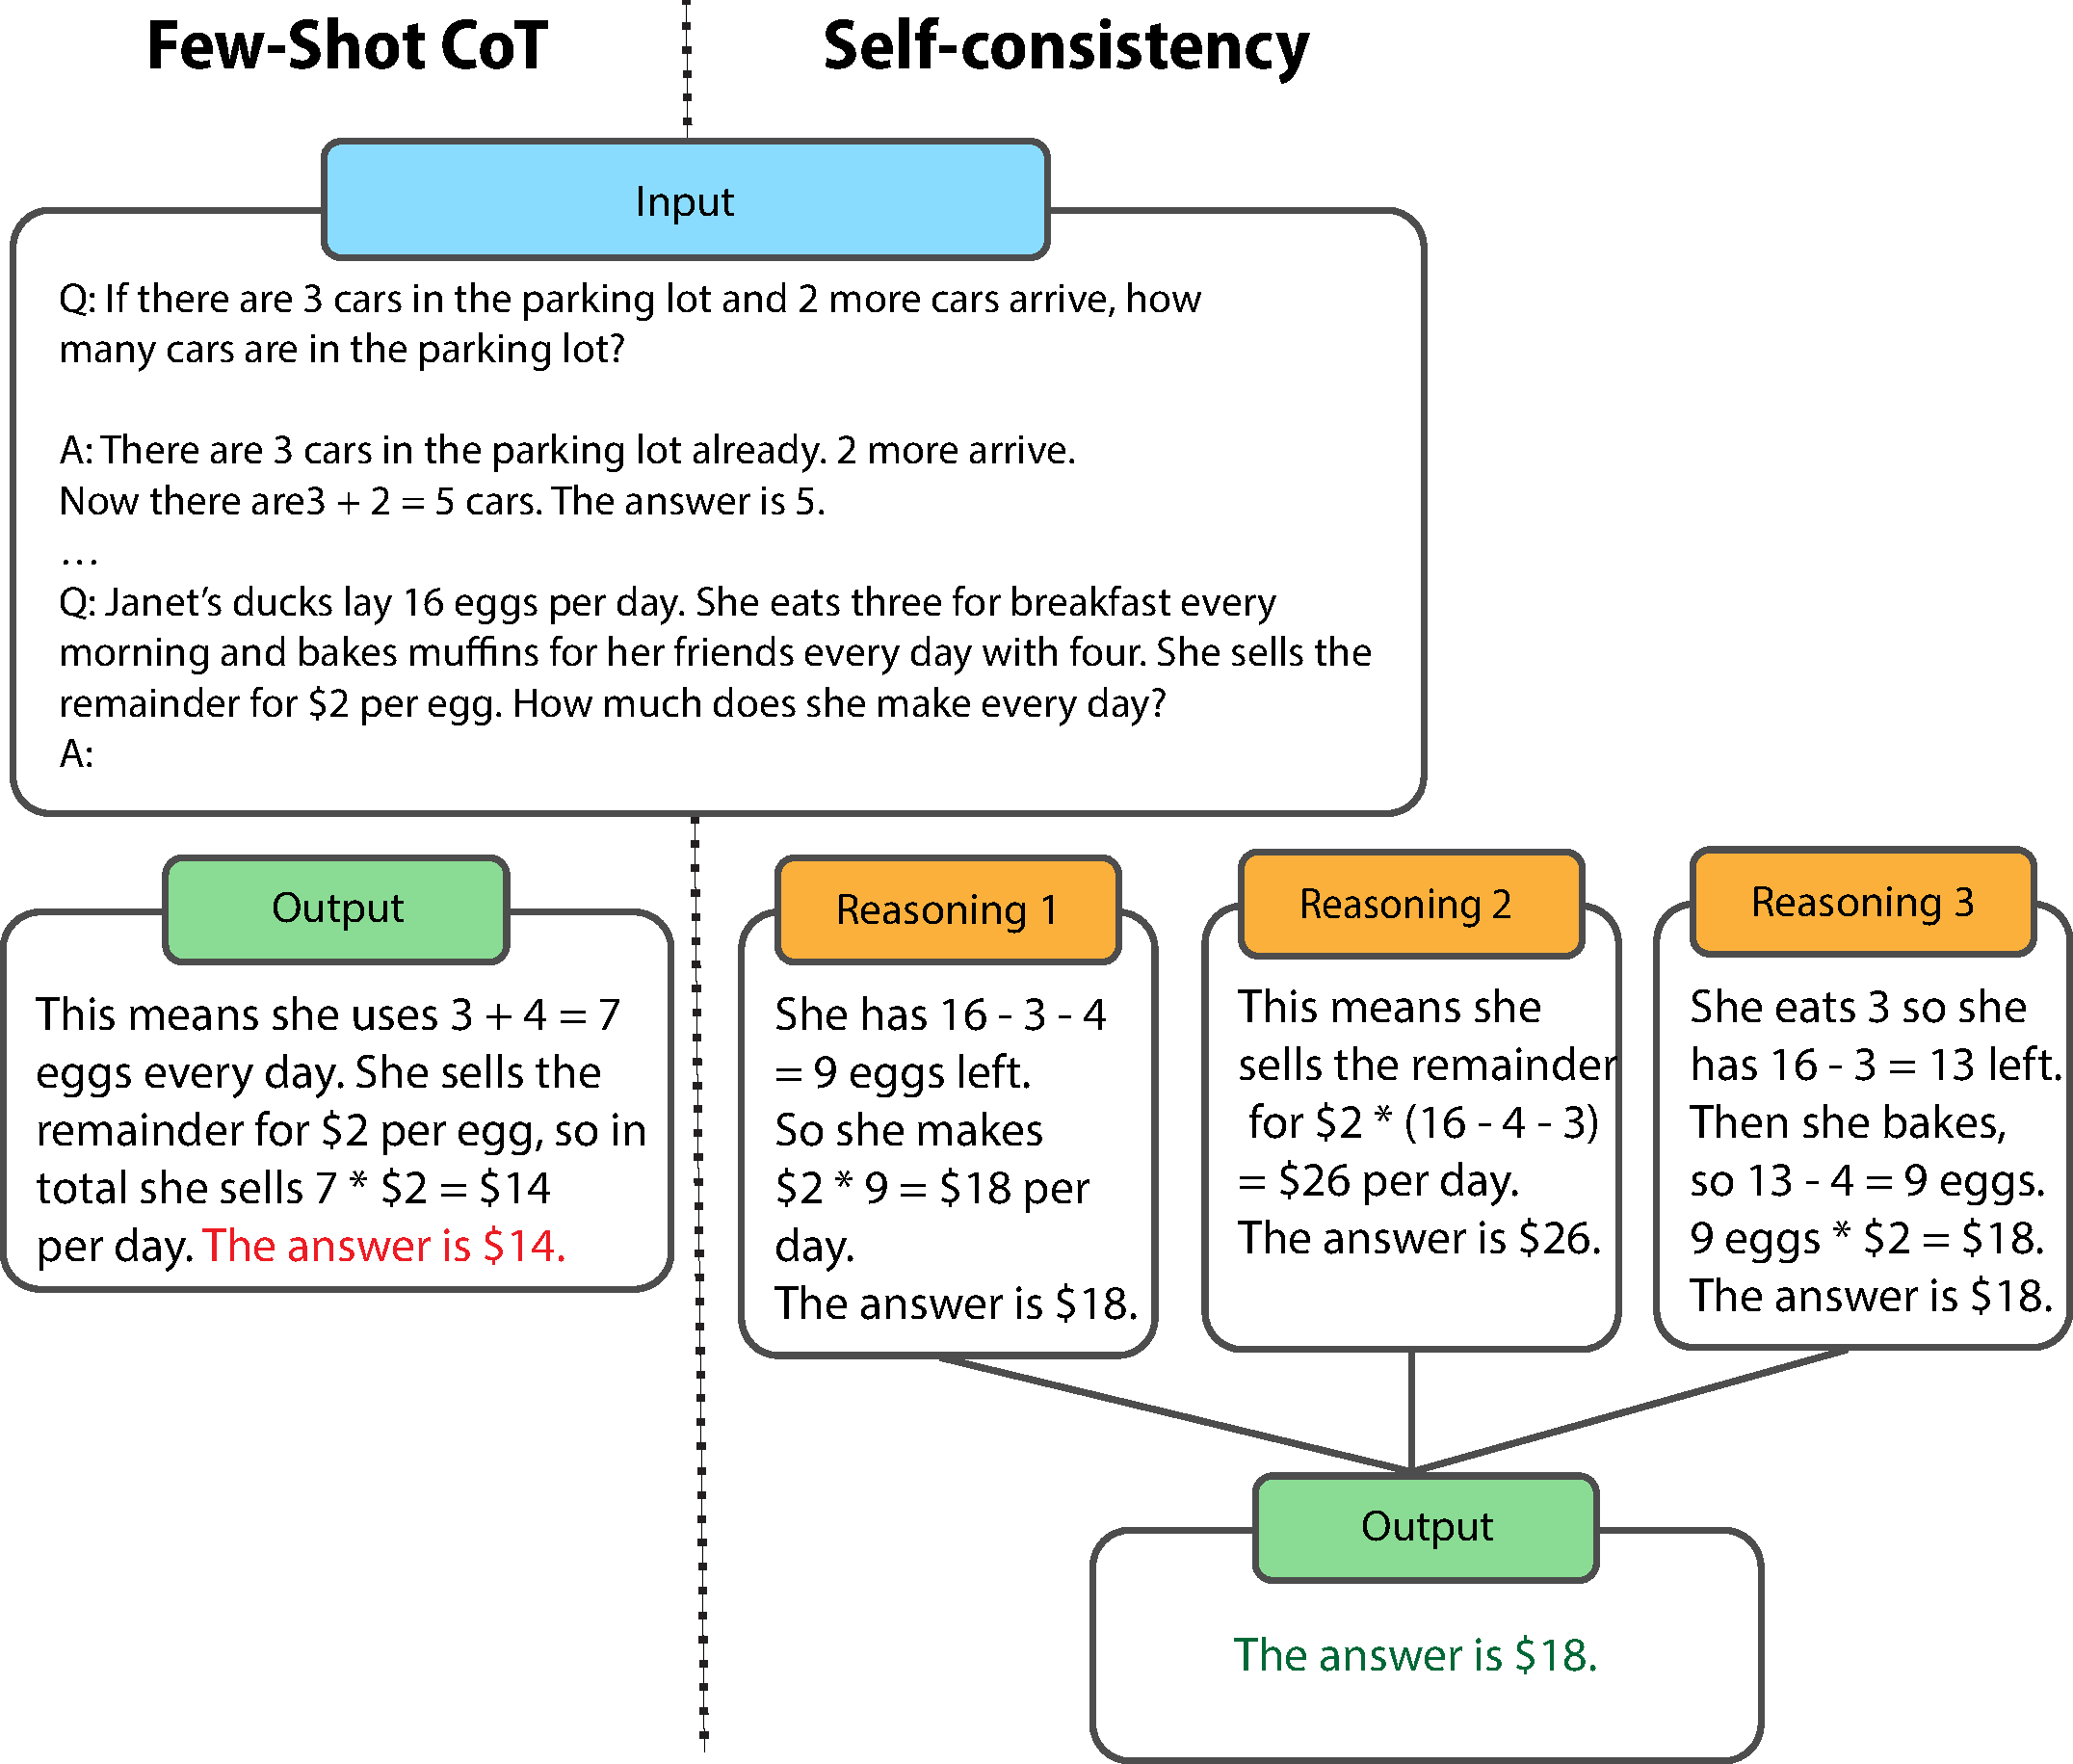
\includegraphics[width=10cm]{figures/selfconsistency.pdf}
    \caption{Self Consistency (Adapted from \citep{wang2022self}),  showing majority voting}\label{fig:sc}
  \end{center}
\end{figure}
%
 
Self consistency has been evaluated on arithmetic reasoning, on commonsense
reasoning and on symbolic reasoning, with a variety of LLMs, including GPT-3.
%It is also compared against sample and rank, beam search, and ensemble approaches.
Self consistency typically improves the performance of chain of thought
by a further 10-20 percentage points. Self consistency  is often used in combination with chain of thought in modern LLMs. % and approaches that we discuss in this book.
%(Self-verification also reports that
%performance is improved when used in combination with Self-consistency
%\citep{wang2022self} and with Program-aided-language \citep{gao2023pal}.)

\subsubsection{Code Generation for Validation}\label{sec:selfdebug}

Another approach to improve the accuracy of a sequence of reasoning steps is to switch from a natural to a formal language. The advantage
of a formal language is that it is less ambiguous than a natural language. Examples are computer languages, such as Python, or mathematical logic. 


%\paragraph{Codex}
LLMs have been quite successful in generating computer code from natural language prompts.
\citet{chen2021evaluating} introduced Codex, a GPT model that
was trained on publicly available  code in the repository
GitHub.  Codex is able to generate correct programs from
descriptions in natural language, such as commentary strings.
%Figure~\ref{fig:codex} shows examples that are produced by Codex.
%
% \begin{figure}
%   \begin{center}
%     \includegraphics[width=12cm]{figures/codex}
%     \caption{Codex example \citep{chen2021evaluating}}\label{fig:codex}
%   \end{center}
% \end{figure}
%LLMs are well suited for generating computer code. 
Subsequently, the use of a formal language for reasoning has become a popular approach. %The work on Codex is used as a basis for further research on reasoning in LLMs.
Many approaches  generate the reasoning steps in Python, so that  the code can  be evaluated by a compiler, debugger, or interpreter.
Human programmers, when writing code, typically
follow a cycle of writing some code, compiling and executing it to look for errors,
and then using the feedback to improve the code. This approach
is followed, for example, in self debugging 
\citep{chen2023teaching}. %Self-debugging teaches a large language model to  debug its generated  program code via few-shot demonstrations. 
It follows the same steps of  code generation, 
code execution, and  code explanation.
%(see Figure~\ref{fig:debug}).
%
% \begin{figure}
%   \begin{center}
%     \includegraphics[width=10cm]{figures/debug}
%     \caption{Self-Debugging control flow \citep{chen2023teaching}}\label{fig:debug}
%   \end{center}
% \end{figure}
 %
Self debugging is able %, without human feedback on
%the code's correctness or error messages, 
to identify mistakes in its own
code %that was generated by itself from 
by investigating the execution
results, and can also provide an explanation of the generated code, in
natural language. %It achieves strong performance: the text-to-SQL Spider benchmark improves 9 points,  and the C++ to Python Transcoder benchmark improves by 12 percentage points. 


%\paragraph{Program of Thought and Program Aided Language}
%Two other approaches that use a formal language are Program-of-thought  \citep{chen2022program} and
Another approach, program aided language  \citep{gao2023pal}, uses the LLM to generate Python and then use an interpreter to evaluate the result. In this approach  the problem is translated into small pieces of Python code, that can then be executed by an interpreter to solve the problem.
%Program of Thought   and Program Aided Language  use the LLM to
%read the natural language problem,  and then generate Python programs as the
%intermediate reasoning steps.
%The approaches are similar although Program-aided-language uses generic prompts, and has been tested on more benchmarks. % and has been used in  other approaches.  
Figure~\ref{fig:pal} (fourth column) illustrates the program aided language approach.
%
% \begin{figure}
%   \begin{center}
%     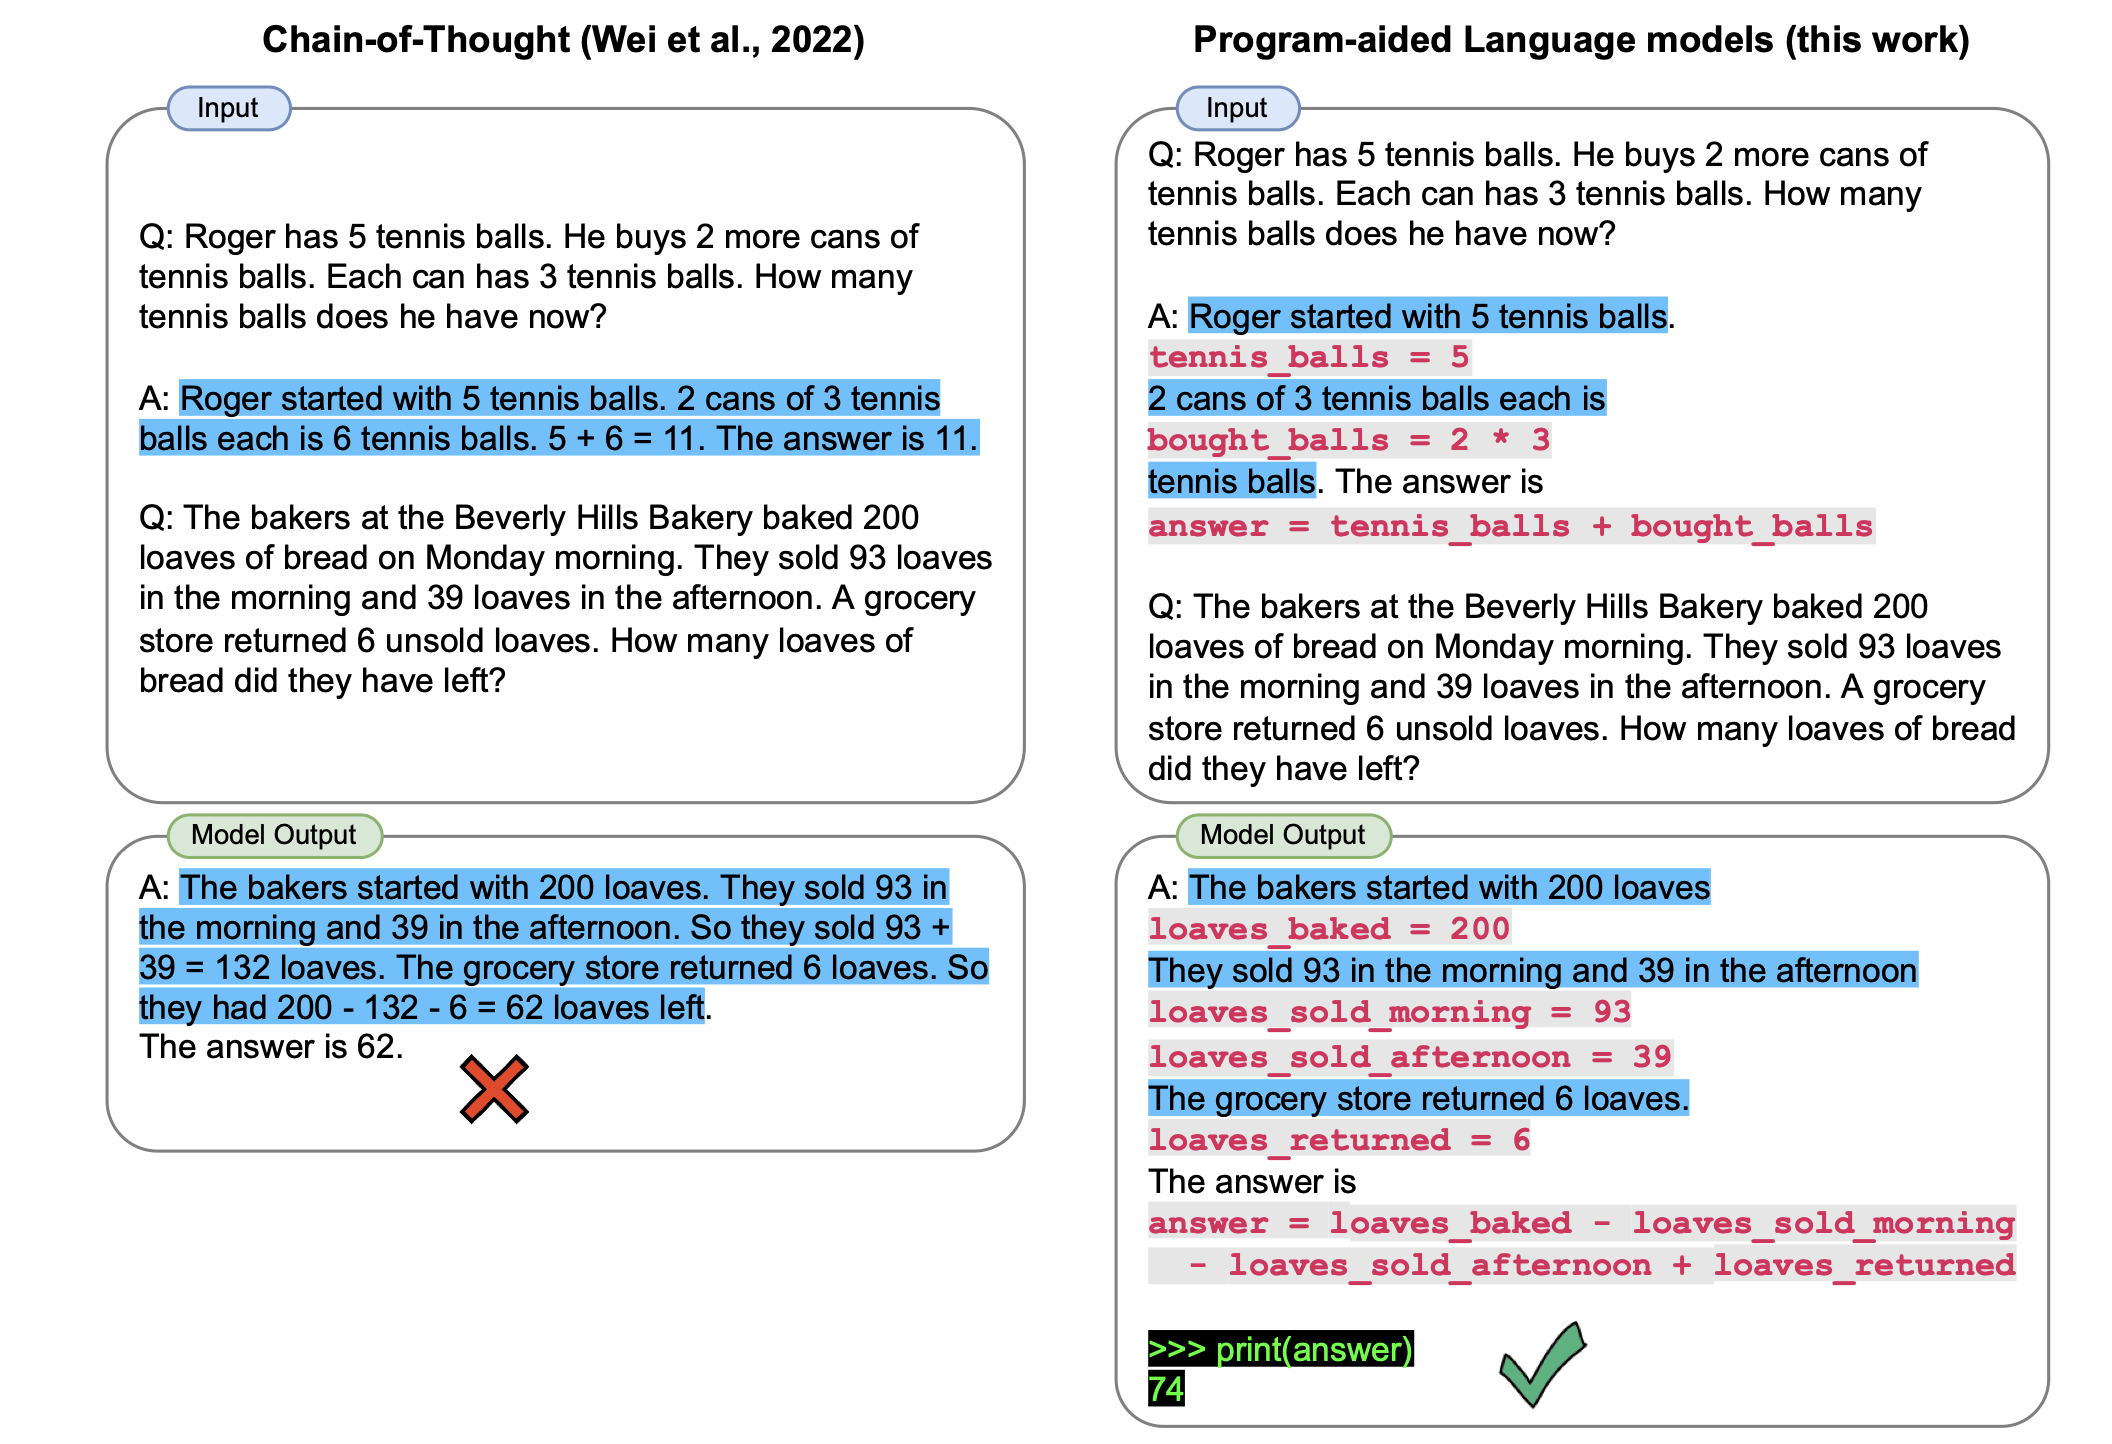
\includegraphics[width=11cm]{figures/pal}
%     \caption{Program-aided-language  \citep{gao2023pal}}\label{fig:pal}
%   \end{center}
% \end{figure}
%
When the evaluation of the reasoning steps is offloaded  to the Python
interpreter, decomposing the natural language problem into executable
code-steps 
remains the only task for the LLM. %(Earlier work in math word problems showed how to decompose a problem and reach an answer \citep{ling2017program}.) 
%
\citet{gao2023pal} provide extensive experimental
evidence showing the synergy between the neural LLM and the symbolic interpreter.
Experiments were performed on 13 mathematical, symbolic, and algorithmic reasoning
tasks, achieving more accurate results than much larger
models of the time (for example, program aided language reported 72\% on GSM8K and  93\% on Penguins). %Mathematical word problems have been studied for some time.  




% FunSearch \cite{romera2024mathematical}
% \todo{FunSearch}

% LLaMEA \cite{van2024llamea}
% \todo{LLaMEa}

\subsubsection{Evolving code generation prompts}
The work on verification with formal languages has lead to several works that generate working code tuned for solving specific problems automatically, without human feedback.
\citet{romera2024mathematical} introduced FunSearch, an approach that integrates formal methods and LLMs to enhance mathematical reasoning and code generation. FunSearch %is capable of producing functionally correct programs that adhere to specified requirements. It 
uses a genetic  approach with multiple populations of candidate solutions (programs), which are  evaluated using a function depending on the problem specification. %In addition to the %problem specification in the form of an 
%evaluation function, also an initial program is given to the LLM in the first prompt. 
After evaluating the  generated programs from the starting prompt, a new prompt  is created, in an iterative fashion, combining a selection of  sampled programs sorted  according to their evaluation score, and the LLM is requested to generate a new program.
Another work  leverages evolutionary computation methods to generate and optimize evolutionary algorithms \citep{van2024llamea}. This approach, LLaMEA (Large Language Model Evolutionary Algorithm),  utilizes LLMs to  design and optimize  evolutionary algorithms. The approach uses LLMs to generate initial algorithmic structures, which are then refined through  mutation and selection. %This  enhances the efficiency of algorithm design, particularly in fields requiring innovative and adaptive solutions, 
Accuracy improvements  on the  Black-Box Optimization Benchmark (BBOB) \citep{hansen2010black}   are reported of 11 percentage points.




\section{Self-Reflection and State}\label{sec:state}
In-context learning has emerged as a powerful new few-shot learning method. When our few-shot examples specify reasoning steps, we can improve the capabilities of LLMs even more. 

In this section we will look at some of the limits of in-context learning,
%. We will analyze what it cannot do, 
and we will look at ways to extend the limits.
%
We will first discuss the question of state and memory. We will look at how state can be passed between separate invocations of LLMs, at long context windows, and at the question if LLMs are good at solving problems for which they have to manipulate state. %We will discuss the ensuing knowing-doing gap, and how improve prompts automatically  by wrapping a simple loop around  the LLM calls. 




\subsection{LLMs are Memory-less Functions}
In-context few-shot learning exploits the capabilities of LLMs to retrieve  knowledge, conditioned by the  prompt. The instructions and examples are provided, and the transformer architecture finds the answer (next token) in its vast model of $(K,V)$-parameters. With chain of thought prompts, the LLM is conditioned on few-shot  reasoning steps that are specified in the prompt. %, possibly translating the reasoning steps to a formal language such as Python. 

In-context learning uses the LLM in a functional way, where all input to the LLM is provided in the prompt. The model $f$ finds the answer $a$ for the input prompt $p$: $$f(p)\rightarrow a.$$
In principle, LLMs do not retain information between LLM calls (model parameters remain unchanged, and there are no global variables with  history). If we wish to refine our request, and we wish to carry state information from the previous call to the next, then all such state must be specified by the user in the new prompt $p'$. The model itself has forgotten all about the previous answer. 

For a chatbot, repeating the entire conversational history in each new question would be a cumbersome and unnatural way of conversing. In human conversation our conversation partners do remember what was last said, without us having to explicitly repeat their last sentence (although, when interviewing politicians, journalists sometimes use this method to try to keep them on message). 
Commercial chatbots  overcome this problem in part using system prompts, by invisibly providing the output of the previous LLM call to the prompt for a new LLM query. However, the principle remains that LLMs are good at finding associative next-token answers for a prompt, but not at all at remembering answers and manipulating the state of variables as we know them from general computer programming languages. As no parameters are changed, LLMs do not remember in-context state between calls.

\subsection{Retrieval Augmentation and Long Context Windows}
The LLM-memory problem goes deeper. All information for the query must be specified in a context window. The size of this context window is limited, which fundamentally limits the amount of information that can be communicated to the LLM for a query. This limitation is a problem % for applications where timely or information from large databases is needed, or 
when a large text (such as a book) is to be summarized. Furthermore, in Section~\ref{sec:icrl} we will discuss in-context {\em reinforcement} learning methods, that work by storing full episode histories in the context window. In short, methods are needed to pass more information to the LLM. 

One of the earliest methods to extend the amount of information at inference time is {\em retrieval augmentation for generative AI} (RAG). RAG lets the LLM place a call to external data, such as a corporate database, or to Wikipedia \citep{lewis2020retrieval}. RAG's use is also in reducing factual hallucinations and providing access to time-sensitive information, such as financial or logistics data. RAG will be discussed in Chapter~\ref{sec:rag}.


For passing longer texts to the model, LLMs have been developed with longer context windows. With the standard transformer architecture, the compute requirements scale quadratically with the size of the context window, and  linear architectures are being developed  \citep{ren2024samba}. Another solution is to compress the information in the context window, for example using semantic compression  \citep{fei2024extending}, by chunking the information \citep{wang2023augmenting,zhou2025mem1}, or by recursive methods \citep{zhang2025recursive}.
Devising novel memory architectures for LLMs is an active area of research  \citep{yan2025general}.

\begin{figure}
    \centering
    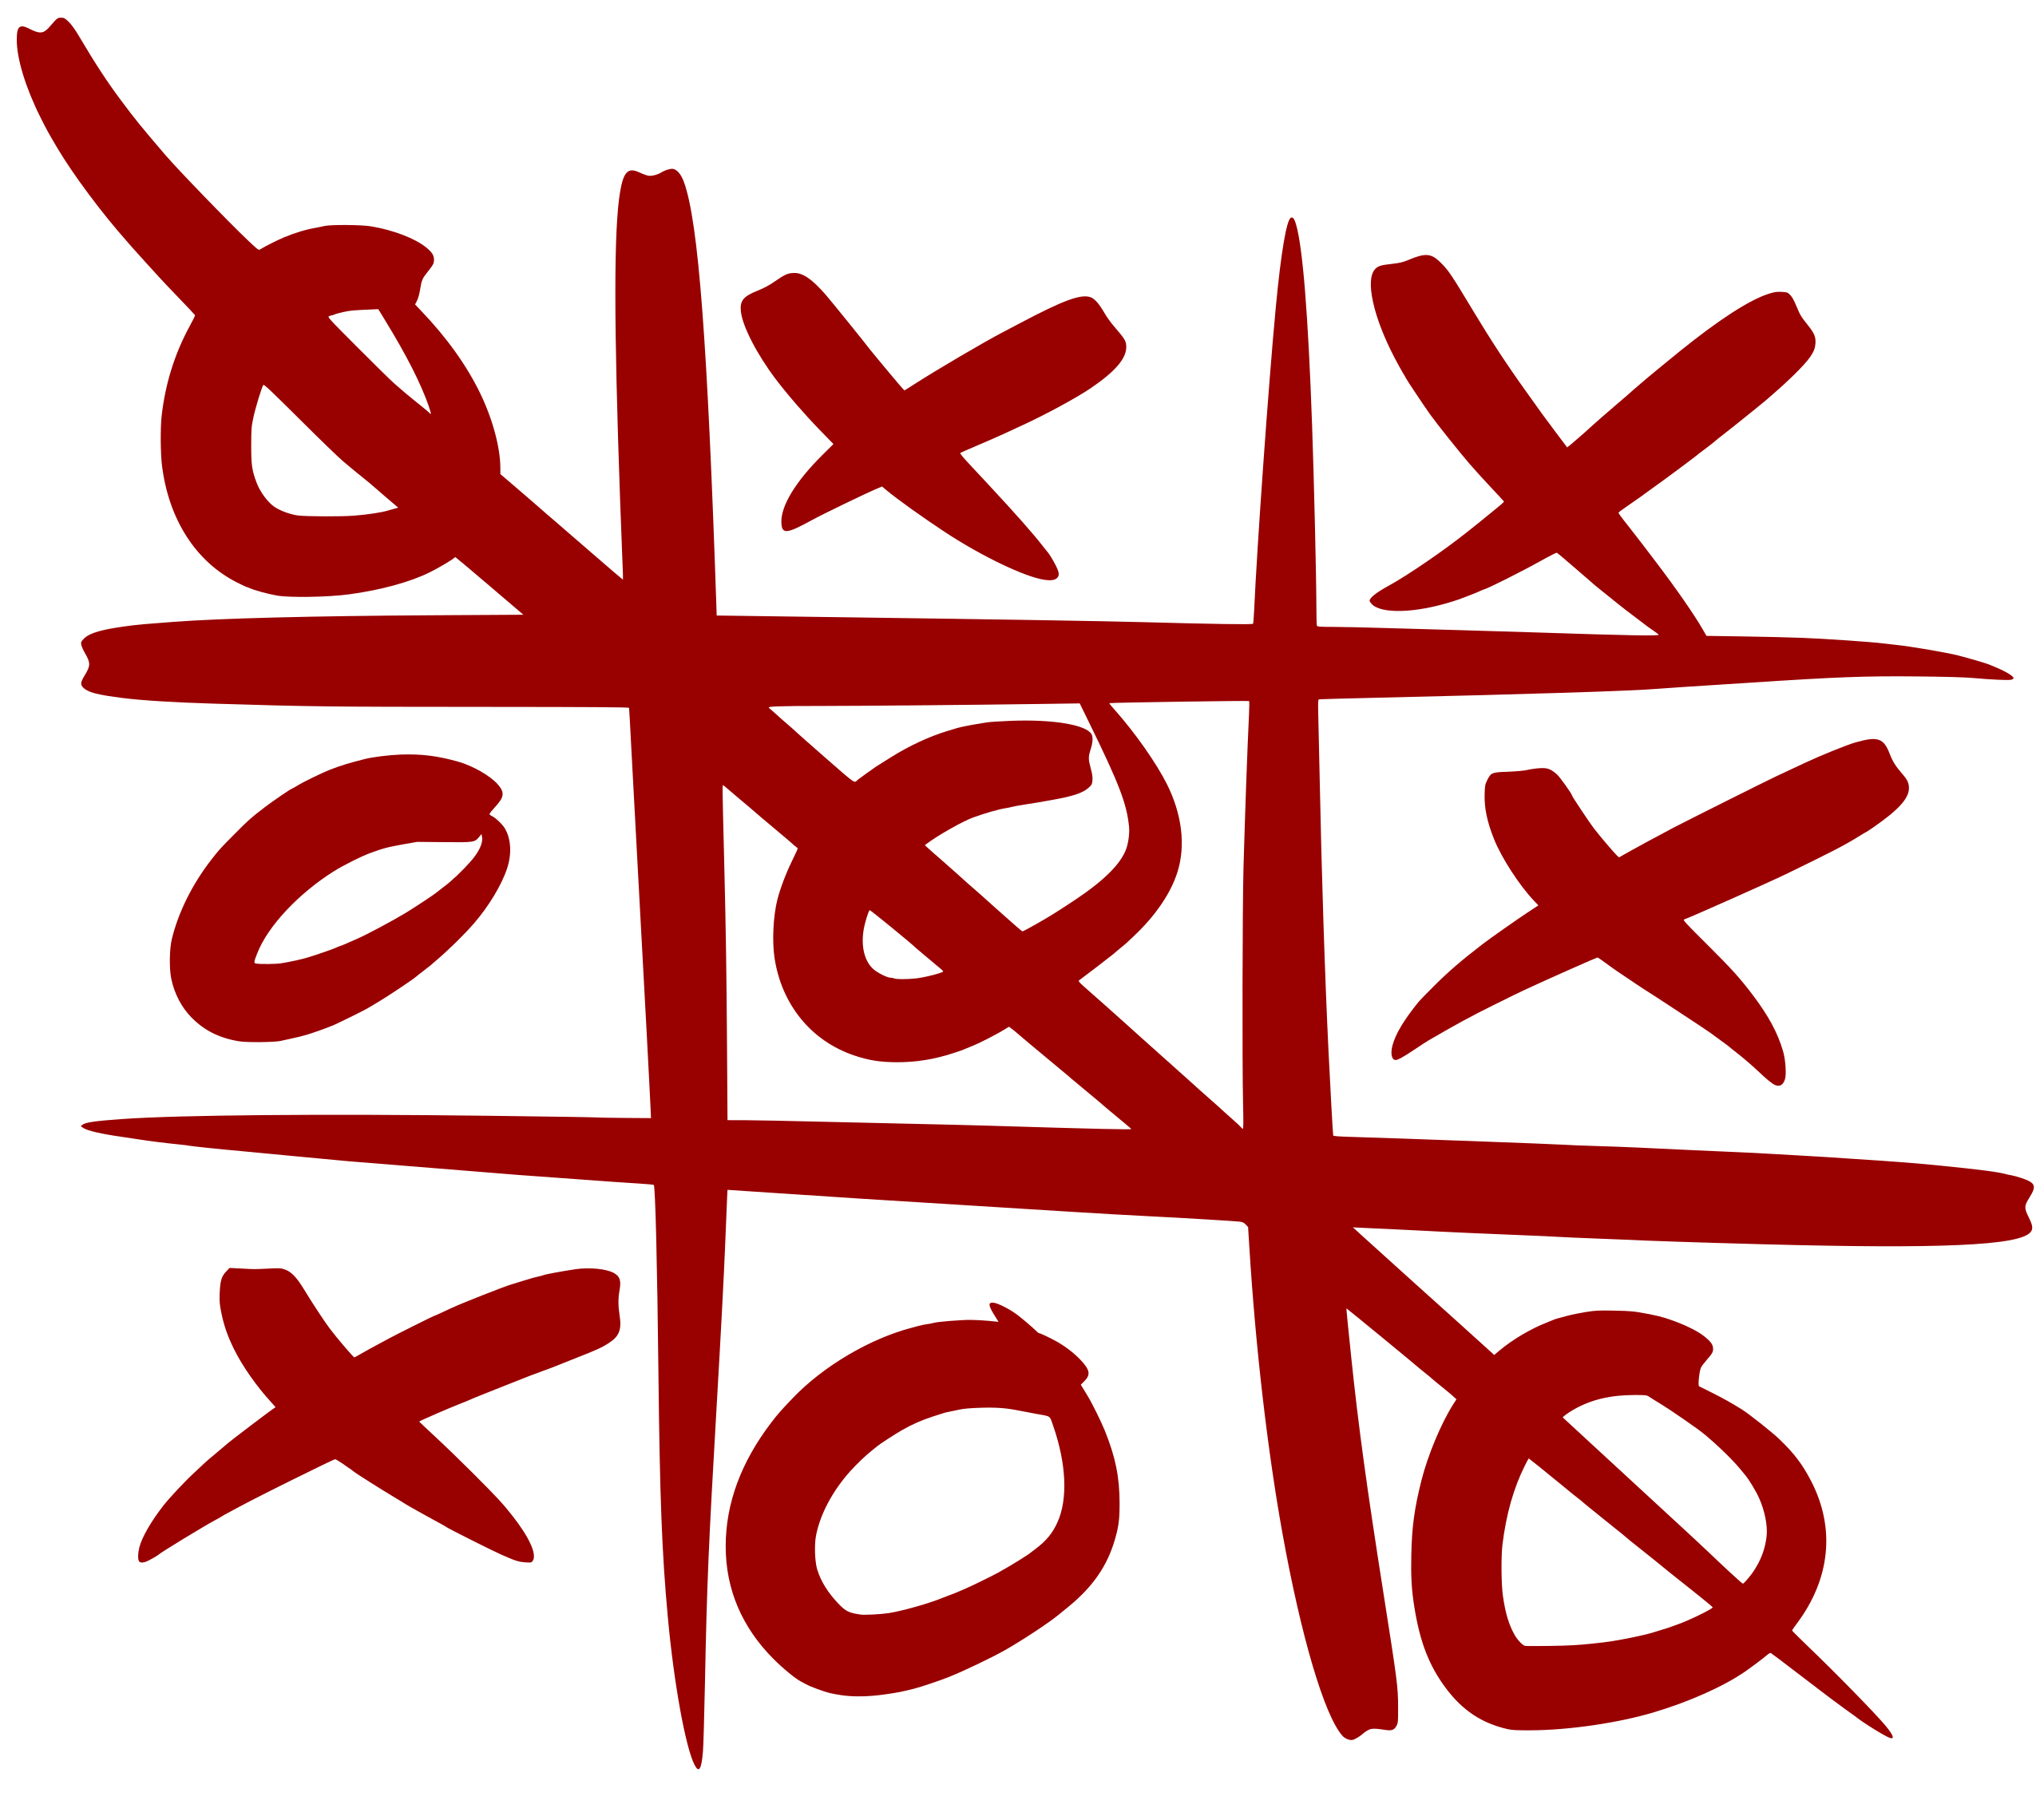
\includegraphics[width=0.35\linewidth]{figures/ttt}
    \caption{Tic Tac Toe is a Simple Board Game, in which State  is important}
    \label{fig:ttt}
\end{figure}

\subsection{LLMs and Stateful Problems}
LLMs perform poorly at solving problems in which state must be managed \citep{wong2025towards}. This occurs for example in planning problems in which the current state has to  be remembered accurately, even  in simple board games such as the one shown in Figure~\ref{fig:ttt}. LLMs tend to mix up the states, and to provide plausible sounding answers that may be correct for games that it has seen in its training corpus, but that are wrong for the actual board state at hand \citep{paglieri2024balrog,ruoss2024lmact}.

Many approaches have been tried to improve reasoning with state,  often inspired by reinforcement learning and planning algorithms \citep{wongstate}.
To see how LLMs can be used to solve these stateful problems, we  discuss how the memory-less nature of LLMs makes them suffer from a problem known as the {\em knowing-doing gap}. %We also briefly discuss if there are theoretical limits to what transformers can do. 
Other, advanced, methods have been developed to  allow LLMs to deal better with stateful problems. Chapter~\ref{chap:arch} will discuss these advanced approaches. 
%First we discuss the idea to pretrain models on decision traces. Next, we discuss methods that optimize prompts externally using search methods, and using learning-based methods, using an agentic harness (self-reflection). %We discuss in-context  reinforcement learning (ICRL), and self-reflection.
%Finally, we discuss implicit reasoning methods. 

\paragraph{Knowing-Doing Gap}\label{sec:knowing}
In addition to the lack of state {\em between} LLM calls, there is another memory-related problem, in the {\em internal}  execution by the LLM of certain tasks. 

This problem  has been named  the {\em knowing-doing gap}. This gap describes the curious phenomenon where an LLM is able to generate a correct textual description  to solve a problem, even the correct algorithm, but is not able to execute this algorithm correctly \citep{paglieri2024balrog}. When you ask an LLM how to solve a certain problem, it can promptly provide the right algorithm in executable Python code. When one subsequently asks it to actually solve this problem, the LLM does not correctly follow the algorithm that it just generated. More often than not, errors start appearing between  state changes of the variables in the algorithm that it generated \citep{paglieri2024balrog,ruoss2024lmact}. Note that faithfully executing algorithmic code step by step, tracking values in registers, is not what the attention-based transformers in LLMs were designed for at all---they were designed to simulate natural language processing through a form of associative memory \citep{la2024code}.\footnote{Note further that the human mind sometimes has the same problem: we can easily describe an algorithm for long division, but when asked to compute $12345/42$, we may make mistakes---computers are good at this, but not humans, and also not LLMs.}

In addition to the knowing-doing gap, there is another state-management problem.
%The $(K,V)$-transformer architecture is good at functional (input-based) associative retrieval, but not at meticulous state manipulation. 
Prompting an LLM to play the first few moves of a board game against itself may show a game in which pieces on the board magically (dis)appear  between moves. The model does not recognize that the moves that it plays that may have been good in certain situations,  do not fit the current board position, and  even decorates these wrong moves with a plausibly sounding reason in a chatty conversational style. %Playing a sequence of moves in a board game, an LLM strings together good moves that it has seen before in similar situations, without critically checking  if the board positions match exactly.  
LLMs have difficulty  reliably managing the state transition of a variable that goes from one value to another value. Individual values tend to be forgotten or mixed up. Additional text can be inserted into the prompt to instruct the model to carefully track values of variables before making a next step \citep{la2024code}, but this is a cumbersome and error-prone solution. %Such extra texts take up valuable space in the context window, and slow down inference. To ensure correct gameplay,  additional text can be inserted into the prompt to instruct it to carefully carry over the correct board state when making a next move.

Both the knowing-doing gap and the disappearing-pieces problem can be circumvented by calling an external interpreter to execute an LLM-generated algorithm. This strategy is sometimes taken by commercial chatbots. It is a smart, practical,  solution, since, in addition to being able to correctly execute Python code, the Python interpreter will do so more efficiently than an LLM. 

Chapter~\ref{chap:arch} will discuss other approaches that address state and memory in the transformer architecture. 

\subsection{Agentic Harness for Prompt Improvement}\label{sec:self-reflection}\label{sec:inferencetime}
%Although decision-trained transformers can solve small planning tasks, losing the ability to converse in natural language with our models is often problematic, and, in LLMs,  the knowing-doing gap for planning problems remains an open problem. 

In addition to resorting to externally executing generated code, other methods have been developed to deal with memory and state. In this section, we will %discuss agentic solutions for state management.
%We will now return to LLMs, to models that are trained on language. 
%We will 
go agentic, and introduce small external algorithms to explicitly manage state and prompts. Such an algorithm is called a {\em harness}. The harness may also call the same LLM in different roles, with different prompts for each role, for example, for {\em generation} or for {\em evaluation} of states. We start with prompt management based on search algorithms. 
%In the next subsections we will see whether LLMs (transformers that are pretrained on natural language) can also do reinforcement learning at test time---in addition to transformers that are trained on decision traces---since it would be convenient to be able to communicate with our agents in natural language. 

When the LLM is called in different roles, for example to critique (evaluate) its own performance (that it just generated), the LLM can be said  to perform {\em self-reflection}. This somewhat anthropomorphic term is often used in the literature for these approaches. Exactly what (not who) is doing the self-reflecting, the LLM, or the agentic harness, is a matter for debate.


\subsubsection{Search-based Prompt Optimization}\label{sec:planning}
%\subsubsection{Self Reflection}
We will now discuss search-based inference-time decision methods.
These are in-context learning methods that go beyond chain of thought. Chain of thought explores a single line of reasoning steps, where each step has a single successor step. Search-based methods  explore multiple options at each step, creating a tree of possibilities. 

When we wish to examine a tree of possible reasoning steps, then we need a method to keep track of the state of which step we have seen, what the best answer so far was, and which steps should still be further examined. As we have seen, LLMs are not terribly good at keeping track of state, whereas conventional computer algorithms, such as small pieces of Python code, are. 
%In reasoning, often multiple valid  steps are possible, but pursuing all possibilities over multiple trajectories may lead to an infeasible number of possibilities. %We can use optimization algorithms to search through the space of possibilities in a smart way. 
%We can use an external prompt management   controller algorithm to do so. 
%For example, 
%Suitable options are standard tree search algorithms or  a reinforcement learning loop algorithm, can be used % to guide the search through the space of possible steps \citep{sutton2018reinforcement,kaelbling1996reinforcement,plaat2020learning}, as a harness. 
%
%\todo{\bf PROVIDE CODE FOR TREE SEARCH AND FOR RL?}
%
%This group of control approaches enables the most elaborate control of the reasoning process, and is used by many works, as we will see. 
Such an algorithm will decompose the problem into a search tree, where multiple alternative steps are
generated that can be searched multiple steps into the future (see Figure~\ref{fig:tot} on page~\pageref{fig:tot}). The  algorithms call the LLM as a subroutine prompting it to perform requested tasks, such as action selection and reward evaluation.  Then, backtracking can be performed by the algorithm, allowing alternative steps to be tried. This control algorithm is external to the LLM. It wraps around the LLM, keeping track of state, managing the prompts, shielding it from the outside world (and shielding the outside world from LLMs that mess up state). The control algorithm is called a {\em harness}. 
%
%Where greedy and ensemble processes can be controlled with a prompt by the LLM, this third category is more complex, and an external algorithm is used to control the reasoning process. 
 %The external algorithm allows more complex reasoning control, but we are now beyond prompt-based self-reasoning: control has been given to an  algorithm that is external to the LLM and external to prompt-learning.

We start our discussion of control strategies with depth-first and breadth-first search \citep{cormen2022introduction}. %then go to beam search, 
%and then to full reinforcement learning.
%
%\paragraph{Breadth first search}
\label{sec:buffer}
%A complex reasoning space can be traversed with a search algorithm.
%Where Chain-of-thought  creates a single prompt with a static sequence of reasoning steps over sub-problems, another approach, 
Tree of thoughts \citep{yao2024tree} uses breadth-first or depth-first search   to dynamically follow different reasoning steps.\footnote{Tree of thoughts is a popular approach. The Huggingface link is here: \url{https://huggingface.co/blog/sadhaklal/tree-of-thoughts}} %When one reasoning path has been traversed, the algorithm can backtrack, and try an alternative path. %The search control is executed with an external algorithm, t
%The paper describes both a breadth-first-search and a depth-first-search controller.
%
Both the generation (red) and the evaluation (green) part in tree of thoughts are performed by  prompting  the LLM, see Figure~\ref{fig:totcode}.
%
\begin{figure}
  \begin{center}
    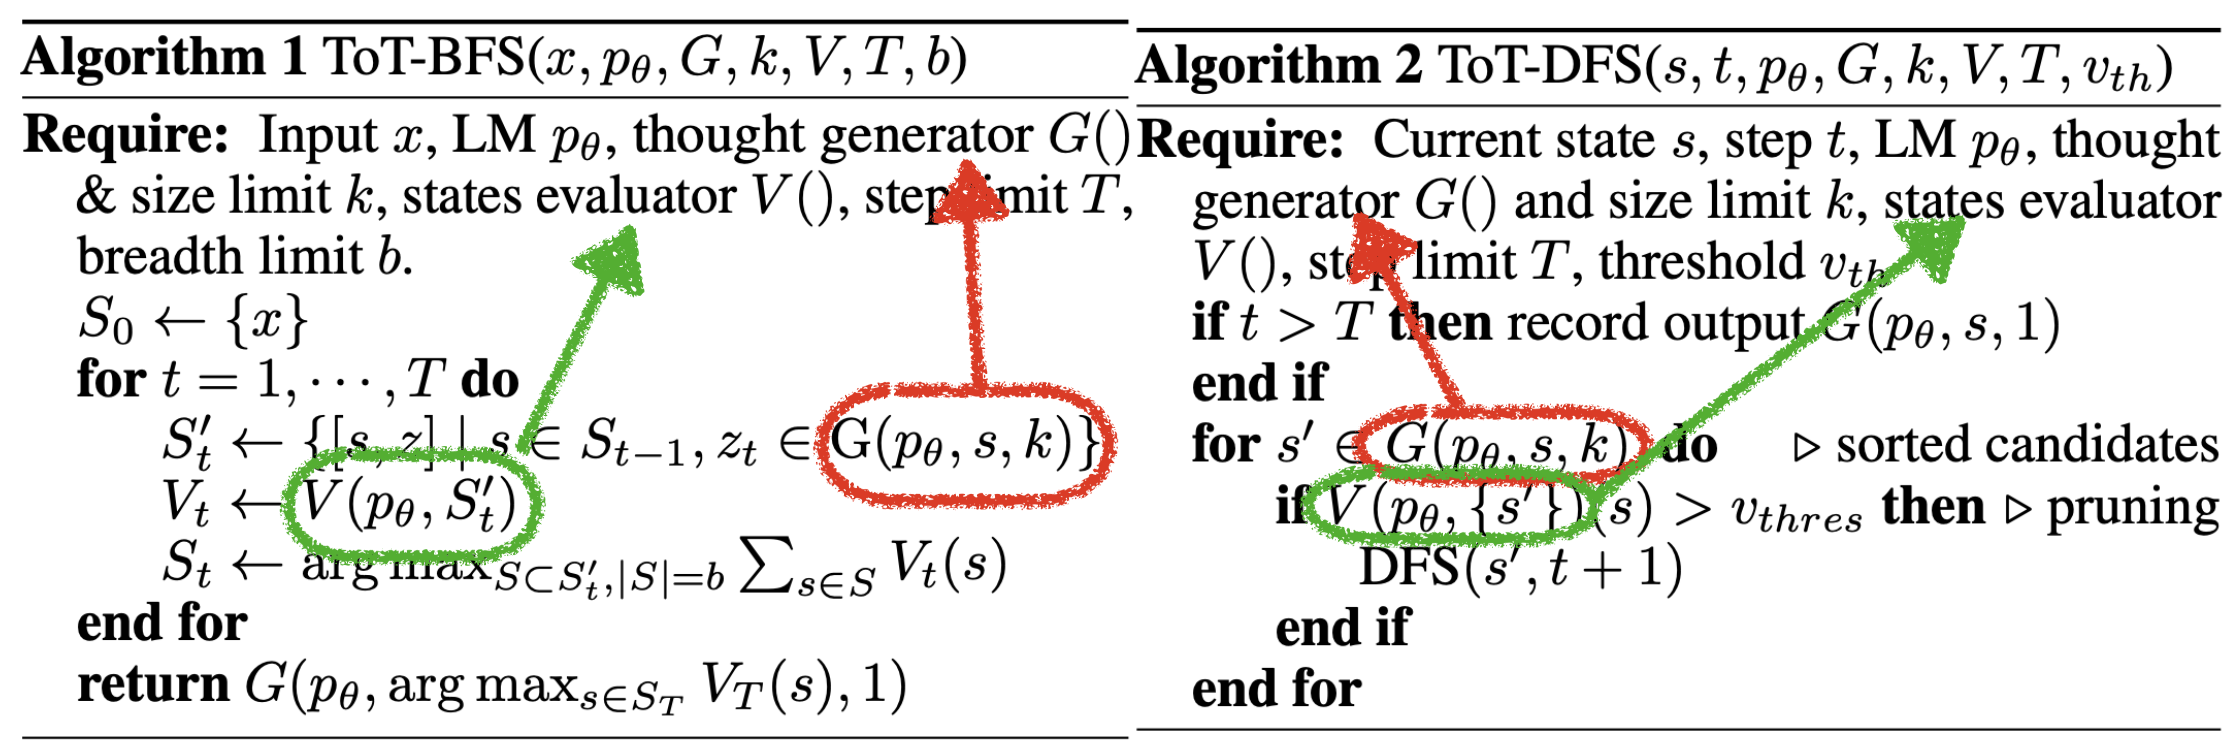
\includegraphics[width=12cm]{figures/totcode}
    \caption{Tree of Thoughts. Left Breadth First Search, Right Depth First Search. The arrows indicate the LLM prompts (after \citep{yao2024tree})} \label{fig:totcode}  
  \end{center}
\end{figure}
%
Together, the two LLM prompts with the external  control,
allow systematic exploration of the space of reasoning steps, performing look-ahead and backtracking. %\todo{Should give example prompts for Generation and for Evaluation for a suitable example game}

\begin{figure}
  \begin{center}
    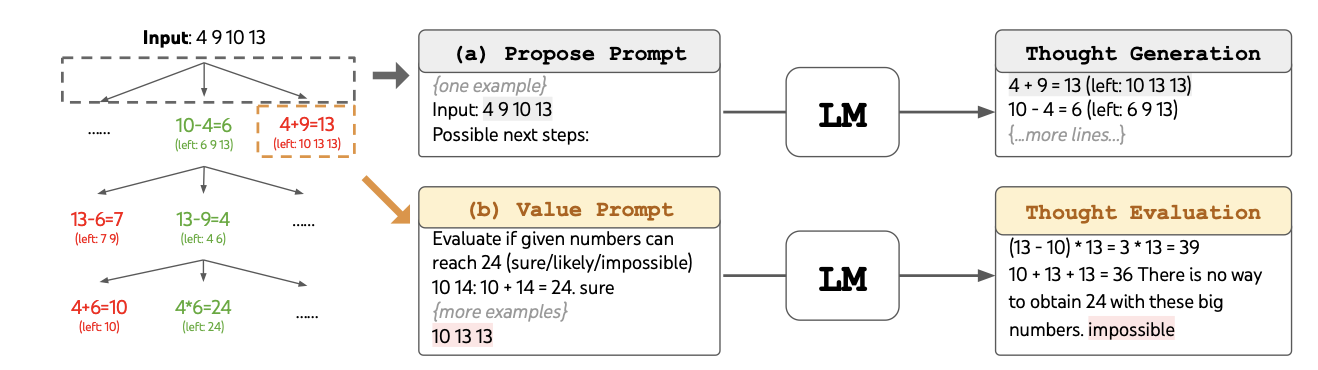
\includegraphics[width=12cm]{figures/tot-ex}
    \caption{Tree of Thoughts Example prompts for Game of 24  \citep{yao2024tree}} \label{fig:tot-ex}  
  \end{center}
\end{figure}

Tree of thoughts (ToT) has been used on planning-based puzzles, such as the Game of 24. In this game, 4 numbers are give, and the task is to reach the number 24 by using the arithmetic operators $( + - * / )$ in between the numbers. For example,  for the numbers $4$ $9$ $10$ $13$, a solution would be $(10-4)*(13-9)=24$. Tree of thoughts first generates a position with the {\em propose} prompt: \verb|Input 4 9 10 13; Possible next steps:| to which the model answers by generating possible next step thoughts. These are then evaluated by the model with an evaluation prompt including chain of thought examples. Figure~\ref{fig:tot-ex} shows a possible  prompting sequence from the original paper. 

The authors compare their approach to traditional linear chain of thought with self consistency on the Game of 24, Creative writing, and Mini crossword, achieving an accuracy of 74\% on a Game of 24 task. The other tasks are evaluated qualitatively. %Chain-of-thought builds a reasoning out of a path of thoughts,
% Self-consistency creates an ensemble of thoughts, and Tree-of-thoughts constructs a tree structure. 
Figure~\ref{fig:tot} illustrates the different reasoning structures.\footnote{A similarly named approach is graph of thoughts \citep{besta2024graph}. Graph of thoughts allows more general reasoning graphs, providing a formal framework, where the different elements can then be specified manually.}

\begin{figure}
  \begin{center}
    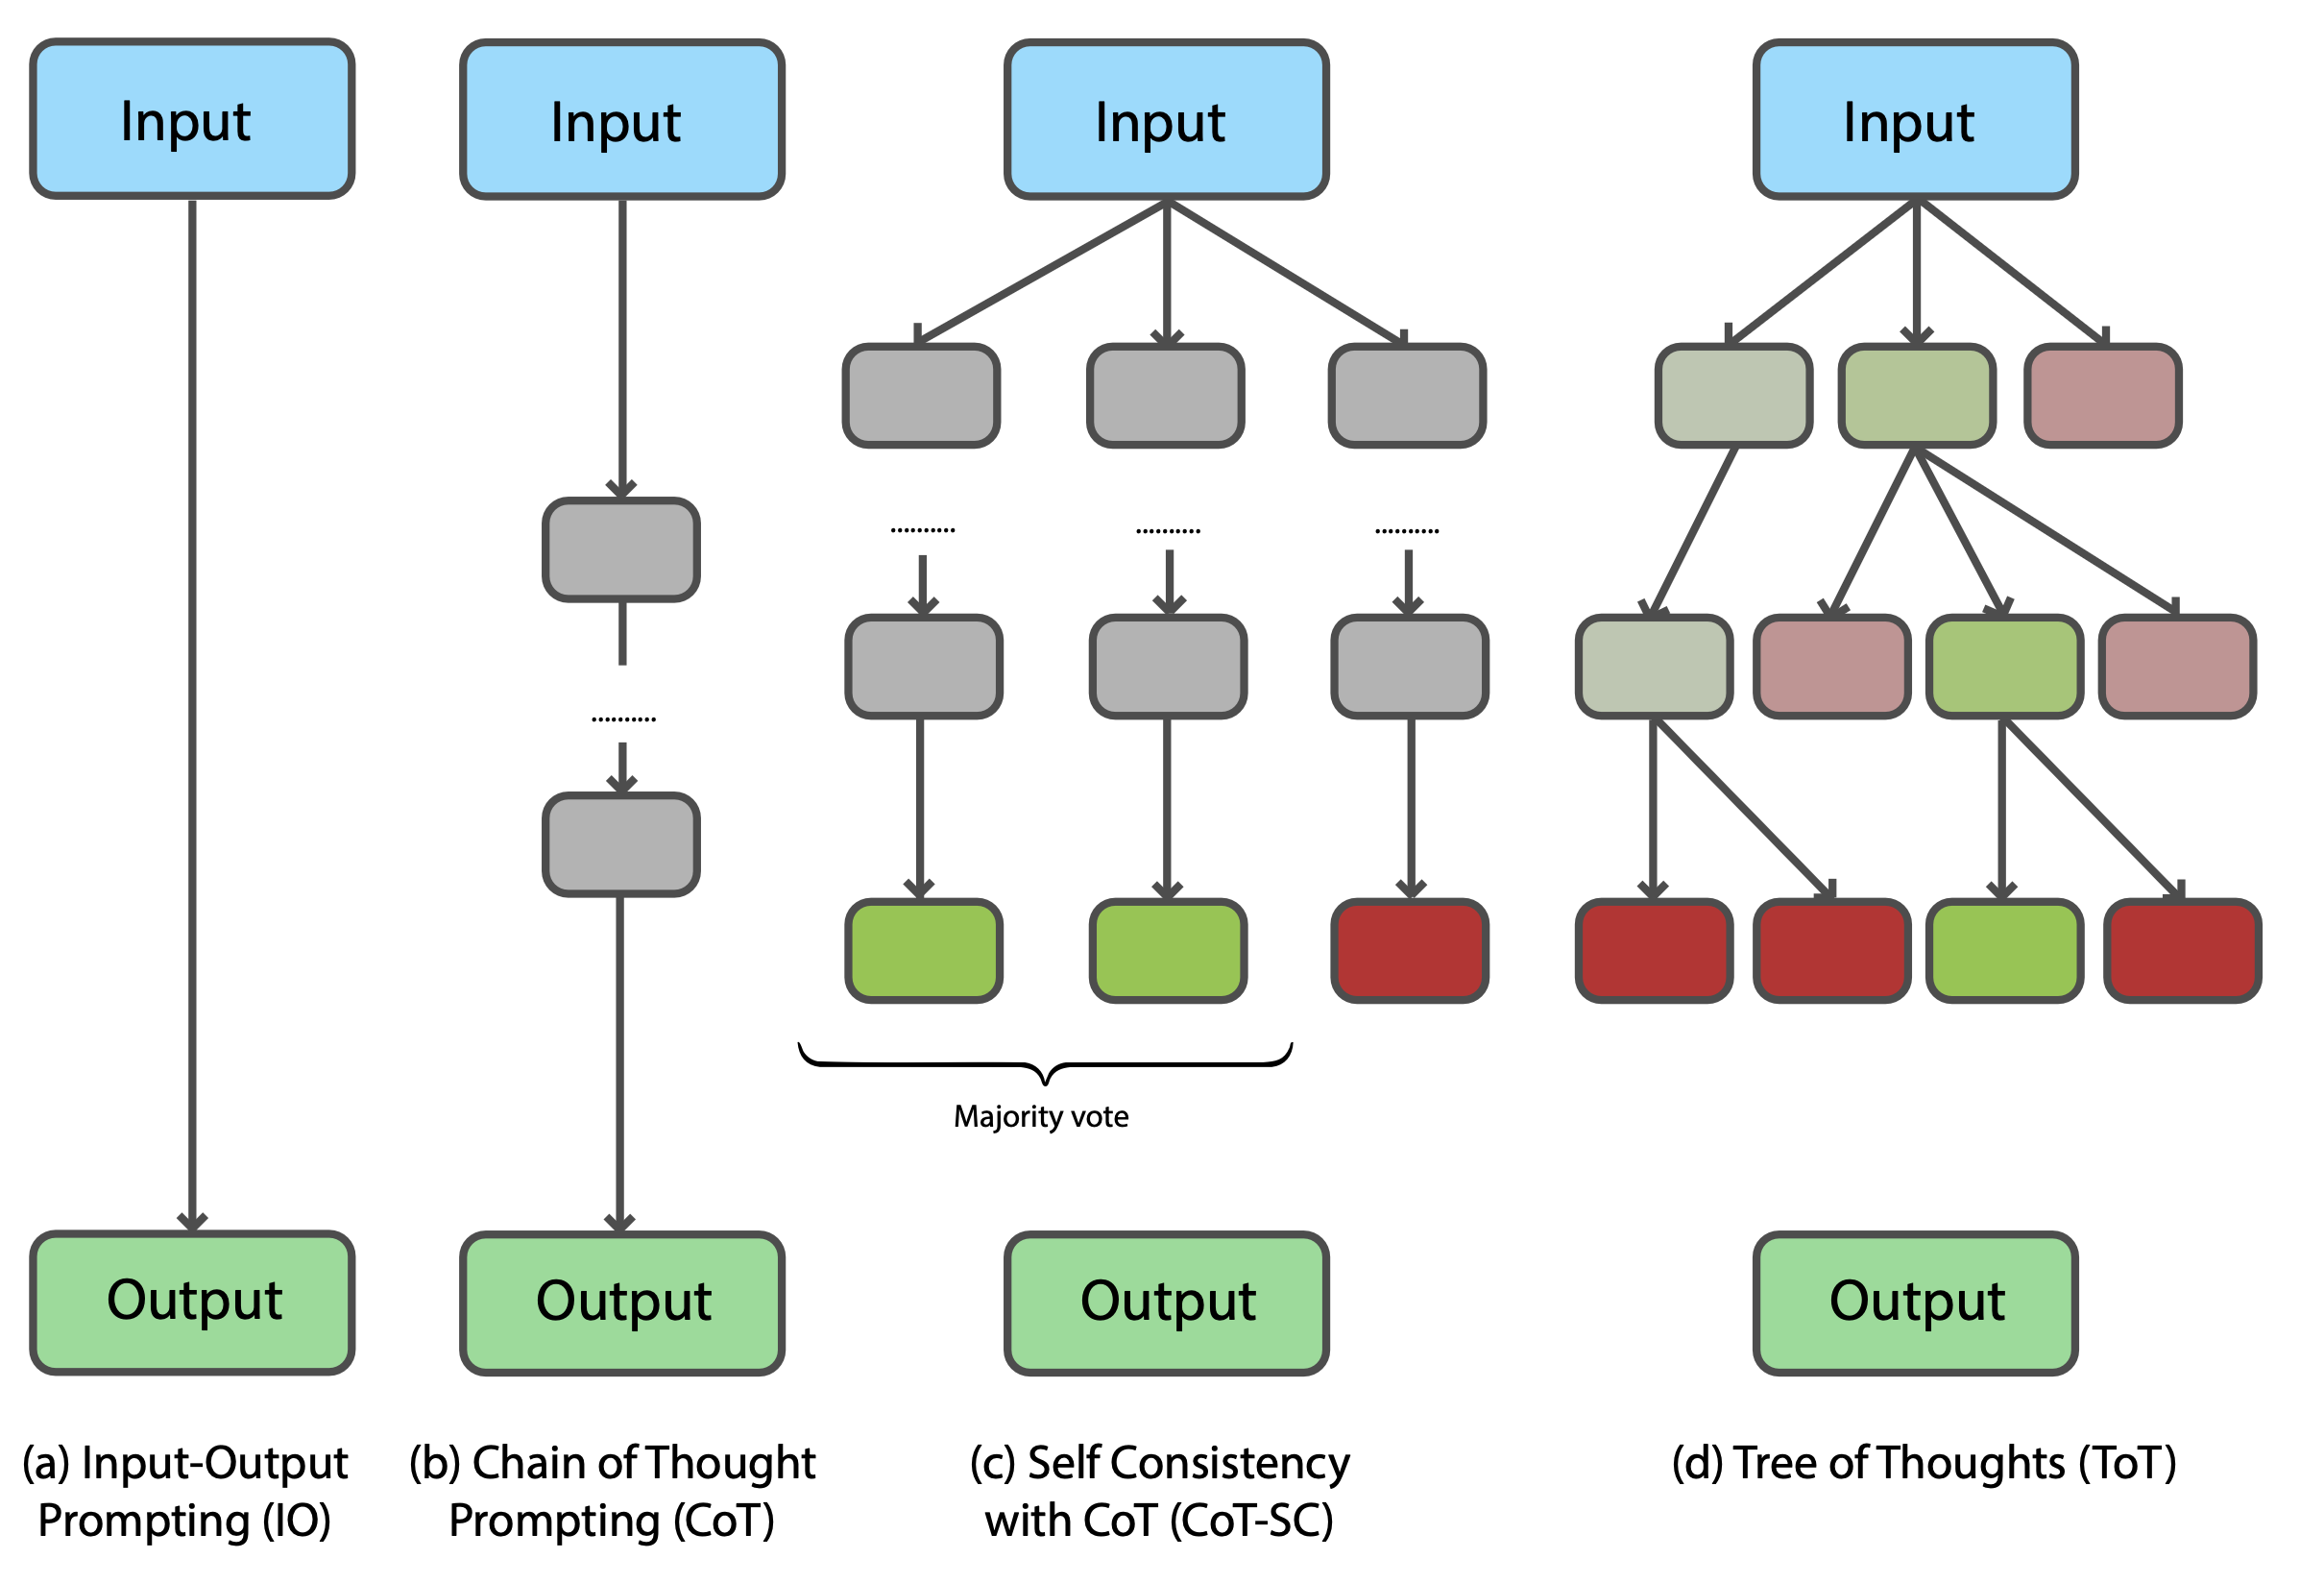
\includegraphics[width=\textwidth]{figures/cot-tot}
    \caption{Reasoning structure of Chain of Thought (b), Self Consistency (c), Tree of Thoughts (d)} \label{fig:tot} \label{fig:bot}  
  \end{center}
\end{figure}

Tree of thoughts is an elegant approach, adding two of the simplest possible search structures on top of an LLM. The sequence of prompts is easy to follow, and finding and correcting mistakes is also easy.  

The two search methods of tree of thoughts follow a  fixed expansion policy. 
Next, we will discuss  more advanced learning-based approaches, that may perform better, at the cost of higher algorithmic  complexity.

\subsubsection{Self-Reflection}\label{sec:reflective}\label{sec:selfreflection}
Many approaches have been devised that use the LLM in more than one role. Such approaches are generally called self-reflective approaches. The LLM is used not just to evaluate a prompt, but also to generate new reasoning steps, and often to refine them. 

The field of self-reflection is young and new approaches are being developed regularly. We will present four such approaches:  self refine,  ReAct, reflexion, and buffer of thoughts. These approaches use the LLMs in different ways, using schemes inspired by reinforcement learning to let the LLMs improve themselves. 

\paragraph{Self Refine} The first %other 
approach is self refine \citep{madaan2023self}. This approach aims to improve answers from feedback. %In this method, initial outputs from LLMs are improved through iterative feedback and refinement. 
%Like PHP, t
The LLM generates an initial output and provides feedback for
its answer, using the LLM to refine itself, iteratively. The LLM is thus used to improve its own answers, see 
Figure~\ref{fig:refine}.
 %and \ref{fig:refine2} 
% illustrates the approach.
% %
% %
 \begin{figure}
   \begin{center}
     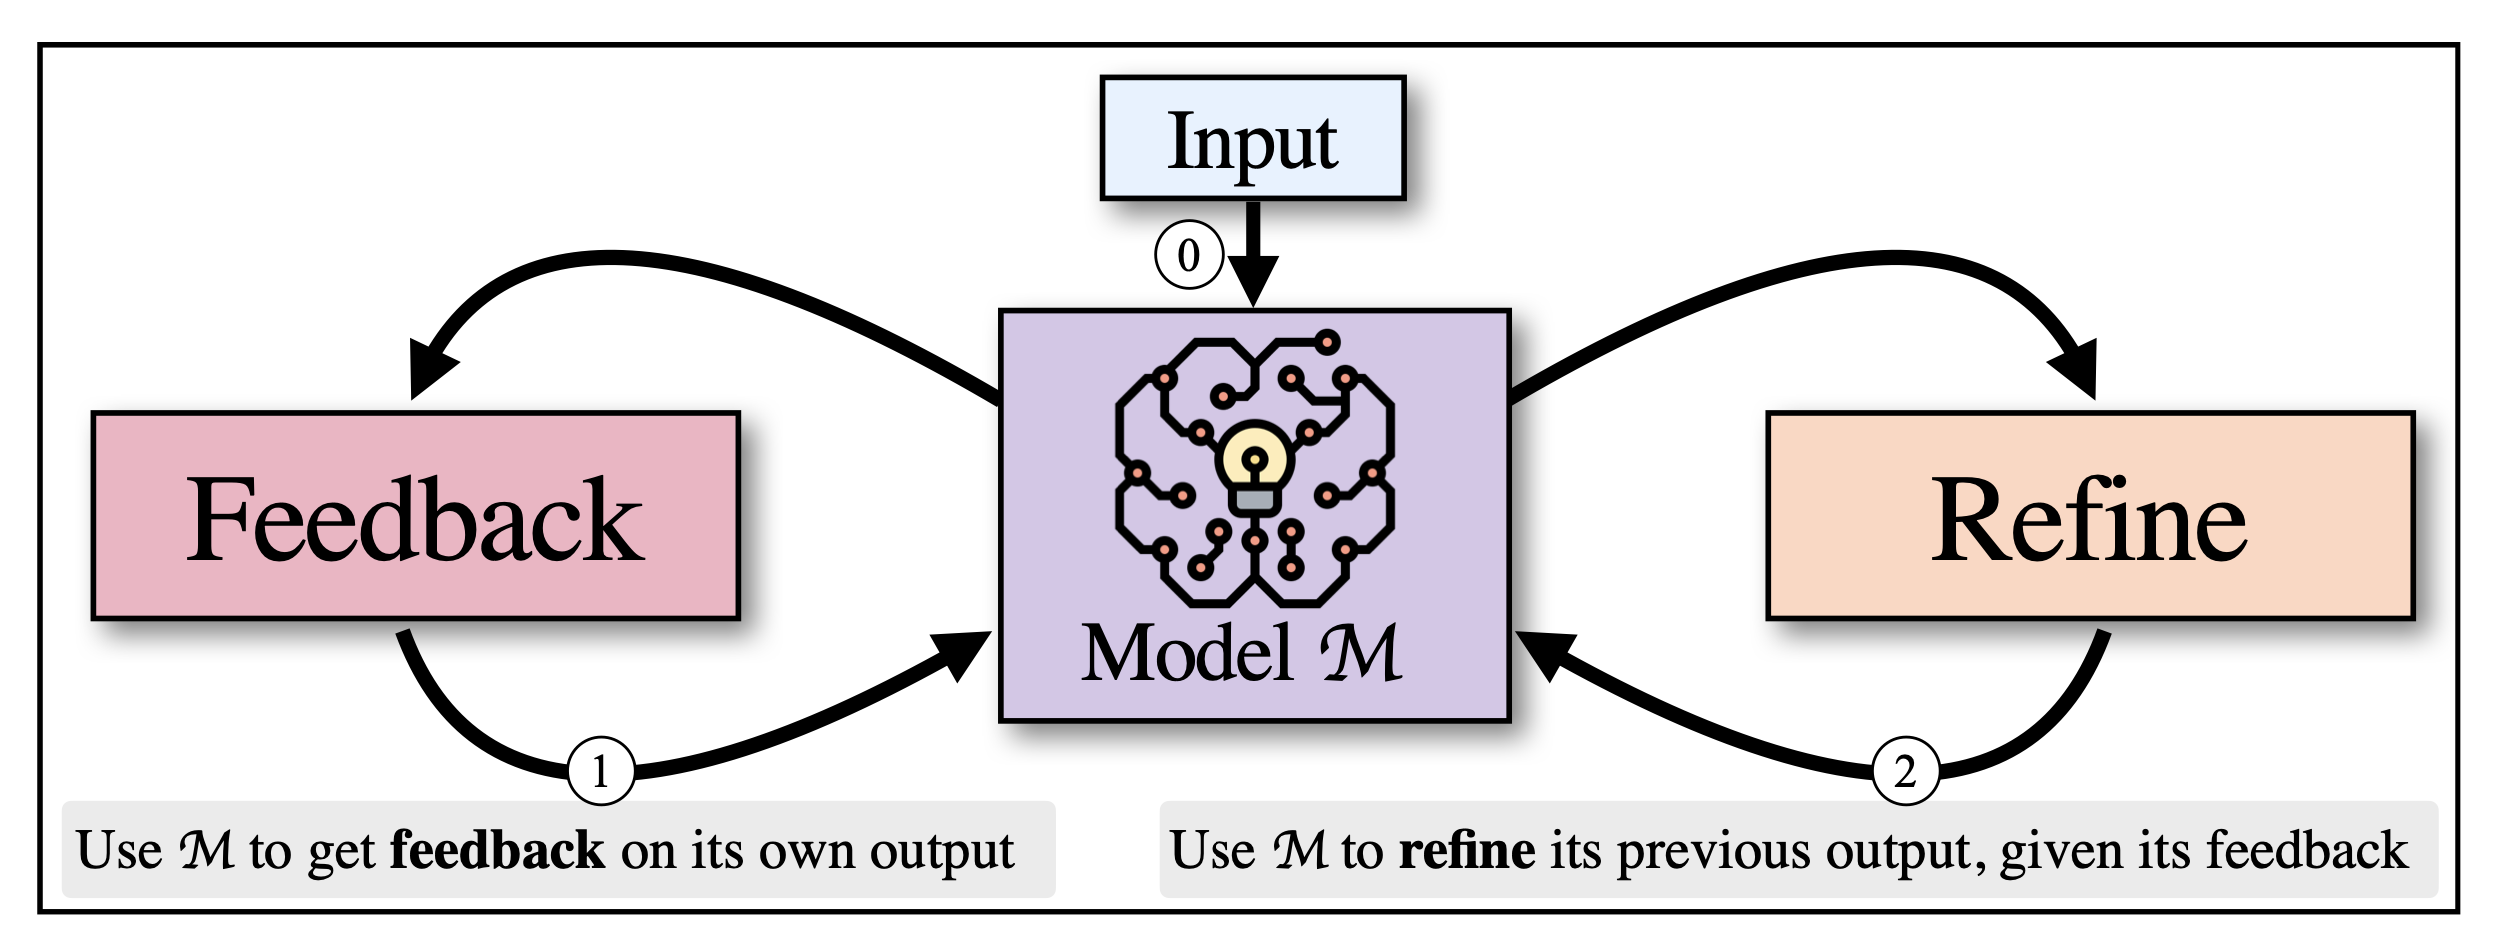
\includegraphics[width=9cm]{figures/selfref}
     \caption{Self Refine Architecture \citep{madaan2023self}}\label{fig:refine}
  \end{center}
\end{figure}
% %
% \begin{figure}
%   \begin{center}
%     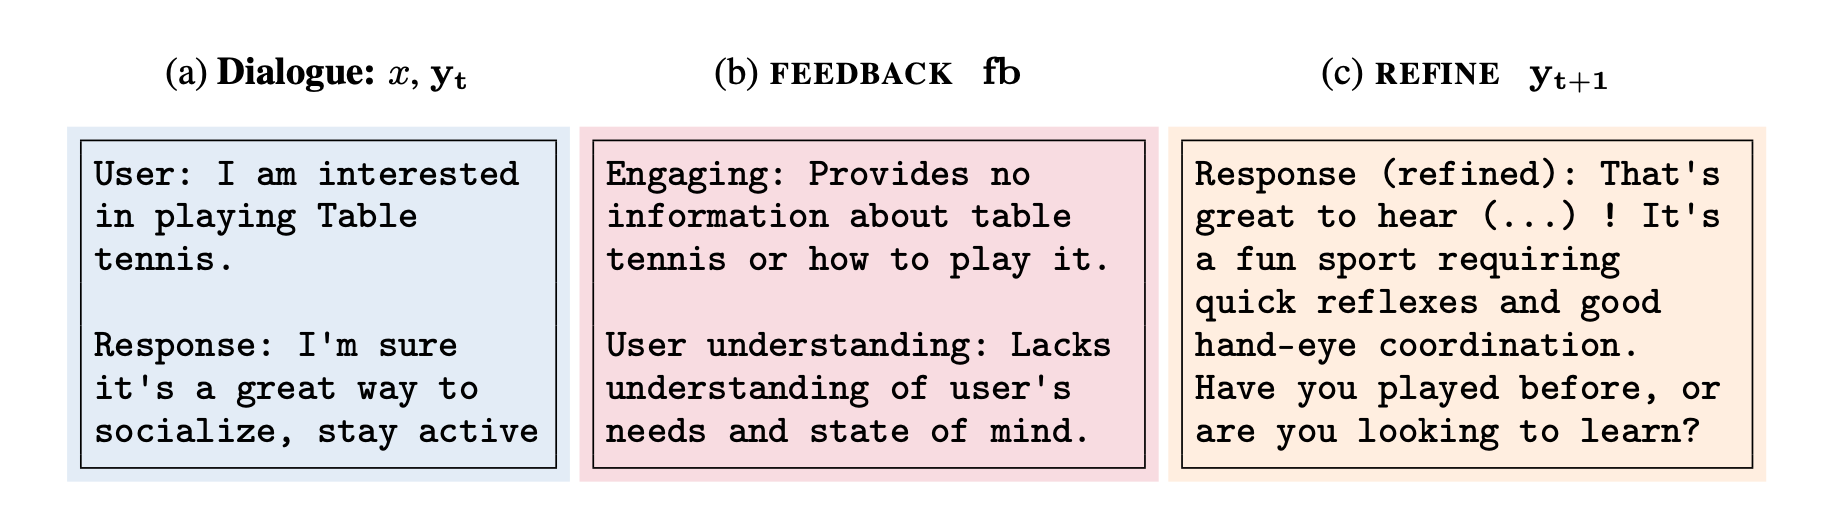
\includegraphics[width=10cm]{figures/selfrefine2}
%     \caption{Self-Refine Example \citep{madaan2023self}}\label{fig:refine2}
%   \end{center}
% \end{figure}
%
%The control flow of Self-refine is again governed by an algorithm external to the LLM and to the prompt. 
Self refine prompts the LLM in three ways: (1) for initial generation, (2) for
feedback, and (3) for refinement, following a greedy reasoning chain.  Self refine reportedly improves significantly over regular chain of thought, on benchmarks such as  dialogue
response generation, code optimization, and 
constrained generation. This approach does follow a linear, greedy, reasoning chain, where a single successor  is tried in a state (it does not explore a tree, as in ToT). 



\paragraph{ReAct}
Generalizing the greedy approach, we can use LLMs to examine multiple options per state.  
A notable approach that combines reinforcement learning and LLMs is ReAct \citep{yao2022react}.\footnote{\url{https://github.com/ysymyth/ReAct}}
ReAct uses chain of thought prompt-learning as part of a reinforcement learning framework that also uses external knowledge sources (Wikipedia) and finetuning; for error reduction, grounding, and for reducing hallucination. The framework allows hand-written prompts.
%, but prompt allows human-written prompts and environment observations.
%
%On question answering (HotpotQA) and fact
%verification (Fever).
%ReAct overcomes 
%hallucination and error propagation in Chain-of-thought reasoning by
%interacting with a  Wikipedia API.
%, and, on the other hand, generating human-like
%task-solving trajectories that are more interpretable than baselines
%without reasoning traces. Furthermore,
% Figure~\ref{fig:react} shows four different
% prompting strategies.
% \begin{figure}
%   \begin{center}
%     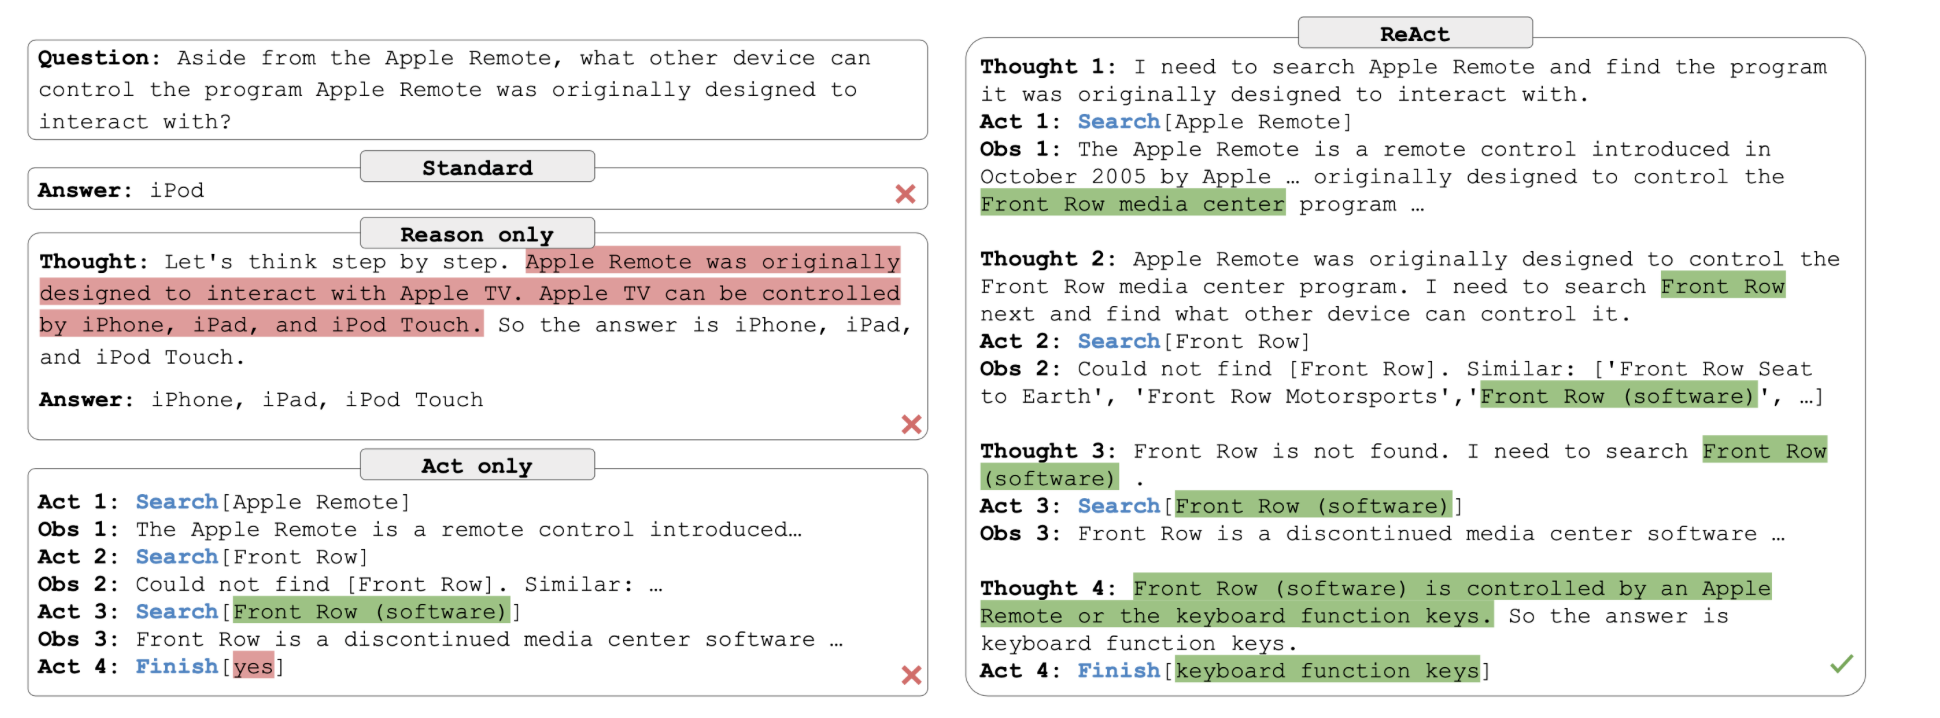
\includegraphics[width=12cm]{figures/react}
%     \caption{Comparison of four prompting strategies: Standard, Chain
%       of Thought (reason), Action only, and ReAct  \citep{yao2022react}}\label{fig:react}
%   \end{center}
% \end{figure}
%
%ReAct also experiments with finetuning of smaller language models
%using a teacher/student knowledge distillation setup.
On two interactive decision
making benchmarks (Alfworld and WebShop),
ReAct outperforms imitation
and reinforcement learning methods by an absolute success rate of 34\%
and 10\% respectively.
%, while being prompted with
%in-context examples. 

\paragraph{Reflexion}
The ReAct work has been developed further.
Reflexion \citep{shinn2024reflexion} %is a system for decision making (reinforcement learning) that 
%is a reinforcement learning system that 
%is built on top of ReAct. %Instead of a neural network with gradients, it is built on an LLM.
%Prompted by Reflexion, the LLM generates actions, to be executed in an environment.
%The goal is to 
creates AI agents that learn by reflecting on failures and
enhance their results, inspired by the way that humans do this.\footnote{\url{https://github.com/noahshinn/reflexion}} 
Reflexion %is implemented as an external algorithm, that 
uses three prompts for the LLM: actor, evaluator, and reflector. 
%A notable extension is that 
The reflexion harness incorporates explicit memory between LLM calls. For trajectory generation it has a short-term memory, and for storing experience information it has a long term memory. This approach addresses the state management problem of regular LLMs using memory in the external algorithm. Reflexion
works as follows: (1) an actor model generates text and actions,
(2) an evaluator model  scores the outputs produced by the actor,
and (3) a self-reflection model  generates verbal reinforcement
cues to assist the actor to self-improve (see Figure~\ref{fig:reflexion2}).
For the actor, chain of thought
and ReAct  can be used. Reflexion has been evaluated on
decision-making, reasoning, and coding tasks. Improvements of 10-20
percentage points are reported \citep{shinn2024reflexion}.
\begin{figure}
  \begin{center}
    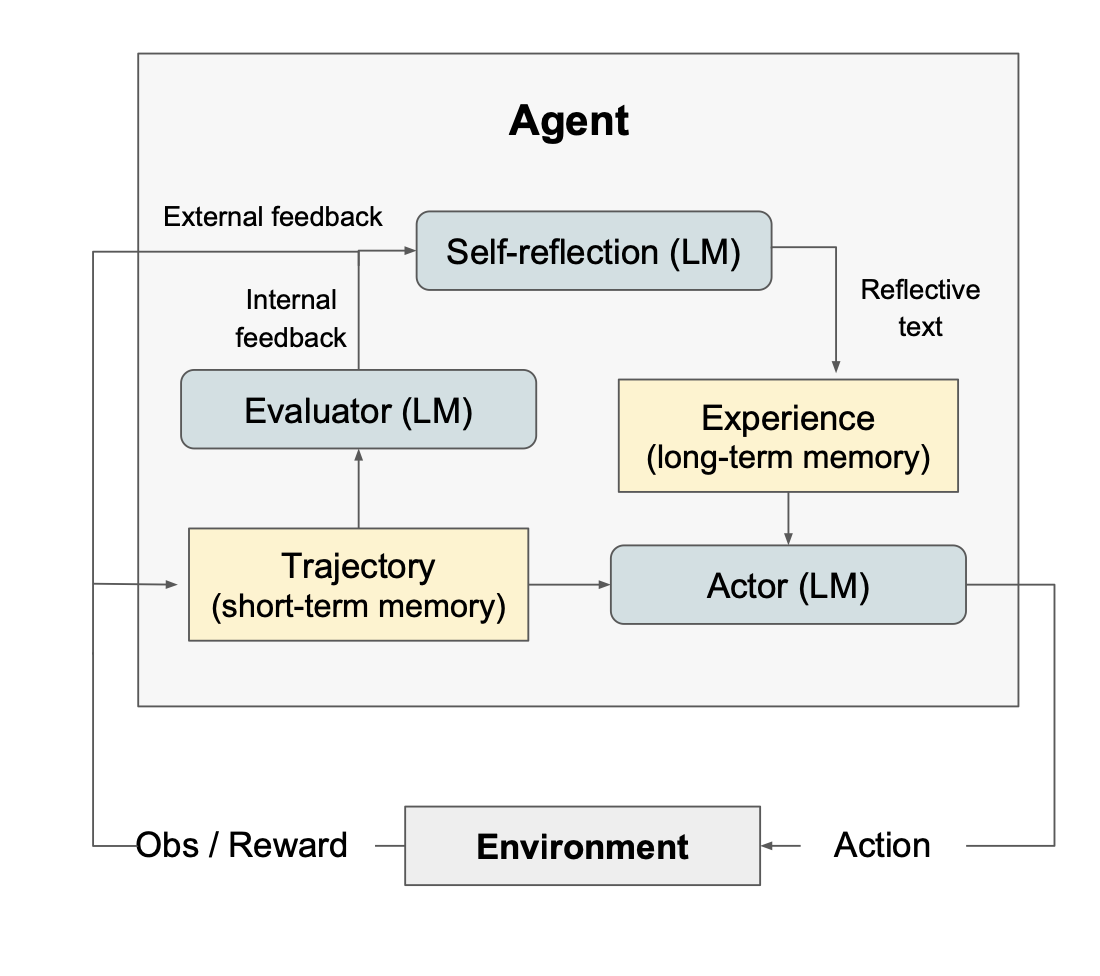
\includegraphics[width=8cm]{figures/reflexion3}
    \caption{Architecture of Reflexion  \citep{shinn2024reflexion}, showing a close resemblance to the agent/environment structure of reinforcement learning}\label{fig:reflexion2}
  \end{center}
\end{figure}
%  Figure~\ref{fig:reflexion} shows three different prompting applications. \begin{figure}   \begin{center}  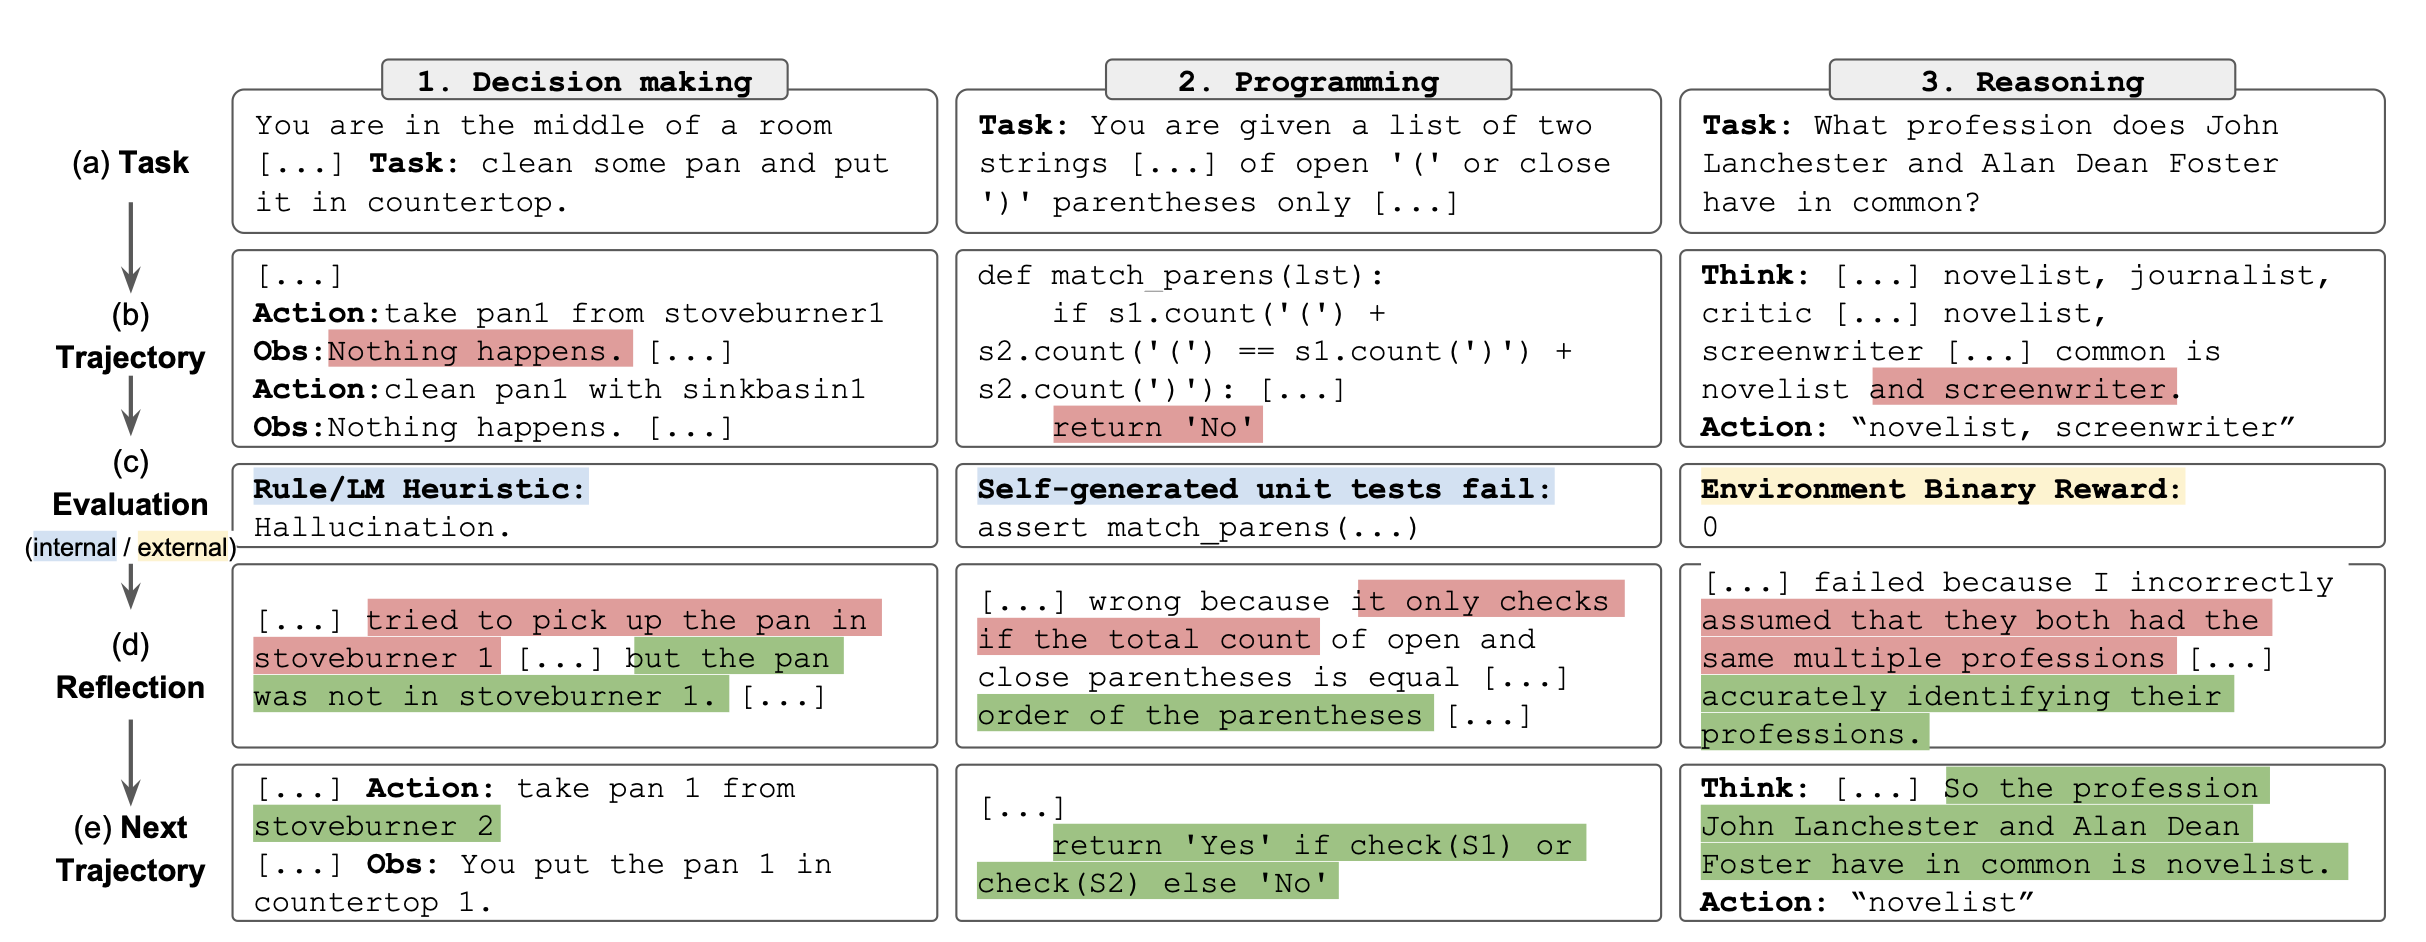
\includegraphics[width=12cm]{figures/reflexion} \caption{Comparison of three application areas  \citep{shinn2024reflexion}}\label{fig:reflexion} \end{center} \end{figure}

%\todo{Provide sequence of example prompts}
%A sequence of example prompts can be in the Game of 24. Reflexion first generates a position with the followin prompt: . It then loops through the possible answers, and evaluates the position with the prompt: . Then, it generates successor positions for each position, that are evaluated.
%\todo{Or do we want to do ReAct, is that simpler and more precise?}
%\todo{Or not, but describe Buffer of Thought?}

\paragraph{Buffer of Thoughts}
Another approach is buffer of thoughts \citep{yang2024buffer}, which goes a step  towards metareasoning \citep{gao2024meta}. It introduces a meta-buffer that stores high-level {\em thought-templates}.  Thought-templates are derived from a variety of tasks. Buffer of thoughts uses a problem distiller that stores high-level
thoughts distilled from different problems in a meta-buffer, which is actively managed for capacity.  Figure~\ref{fig:bot2} compares the buffer of thoughts approach to other approaches such as chain of thought and tree of thoughts. Buffer of thoughts outperforms other methods in puzzles such as Game of 24 (by 11\%) and checkmating (by 51\%). 
%
Thought templates are related to metacognition (thinking about thinking) \citep{didolkar2024metacognitive}. 
%
 \begin{figure}
   \begin{center}
     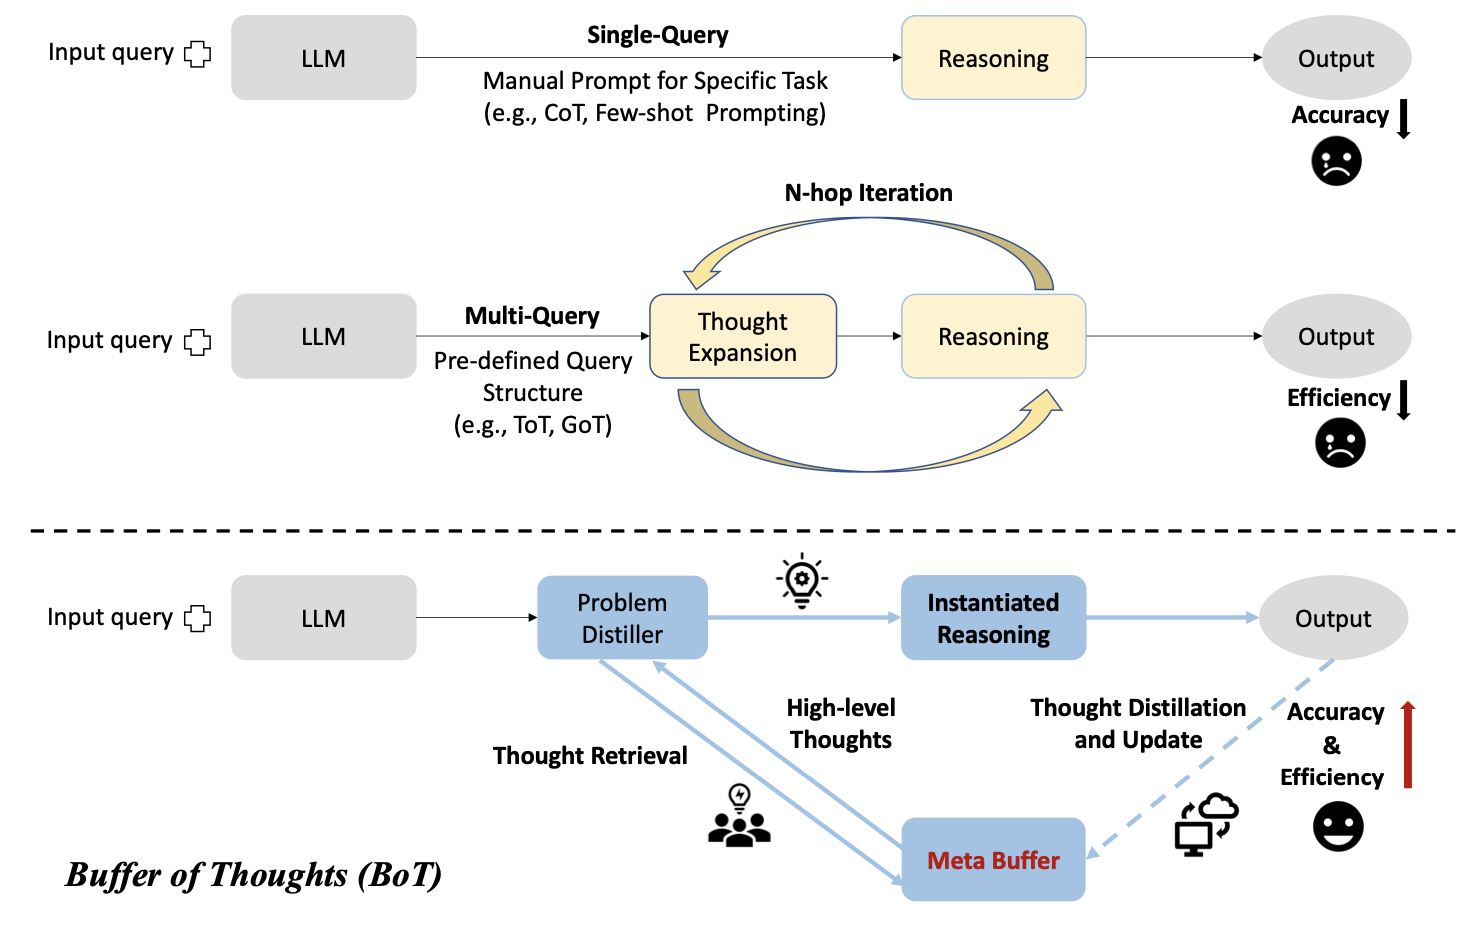
\includegraphics[width=10cm]{figures/bot}
     \caption{Buffer of Thoughts  \citep{yang2024buffer}}\label{fig:bot2}
   \end{center}
 \end{figure}

 


\paragraph{Critique and Prompt Sensitivity}
The concept of self-reflection is not without pitfalls and criticism. To start, the basic idea of asking a model to refine its results begs the question why the model did not give the better answer in the first place. Next, studies by \citet{huang2023large,shojaee2025illusion} find methodological issues with some of the studies, such as the use of data labels that reveal the answer, second refinement prompts that unintentionally reveal more information than the initial prompts, and the use of the same LLM for agent and environment. In one reproducibility study performance did not exceed that of chain of thought with self consistency \citep{huang2023large}. LLMs are  sensitive to how a question is formulated in the prompt. Self-reflection is still a young and active field of research, with an appealing premise, but many open questions. 

The approaches that we have presented potentially make many LLM calls, which can become expensive and slow. Finding the optimum approach for your problem may require quite some experimentation. In Chapter~\ref{chap:balrog} we will discuss a practical case study where we will get hands-on experience with self-reflection methods. Please keep the preceding critique in mind.


\subsubsection{Reinforcement Learning with Verifiable Rewards}\label{sec:rlvr}
The focus of this chapter is on in-context learning. In-context learning occurs at inference time, and no parameters are trained or changed. Finetuning occurs at training time, and does change the parameters of the model. In this section we will, however, briefly talk about a mix of finetuning and in-context learning,  we will be mixing training and inference.

%We  do so because  algorithms have been developed that use inference time results for training purposes. 
%, interleaving inference and training.


Reinforcement learning with verifiable rewards refers to an algorithmic approach for training
language models on tasks with verifiable outcomes such as mathematical problem-solving and instruction
following. Especially for reasoning problems, such as math word problems and coding, inference-time chain of thought results have been found to significantly improve models when they are used for finetuning.

RLVR is an improvement over reinforcement learning from human feedback (RLHF), dispensing with the need for human feedback. In many domains, such as mathematics, a simple function exists to check if an answer is correct, without the need for human feedback. RLVR leverages the existing RLHF objective but replaces the reward model with a verification
function. RLVR samples completions
from a policy model given a set of prompts, and verifies their correctness using a deterministic function. If correct, the reward is positive, otherwise it is 0. This reward is then used to train against using PPO \citep{schulman2017proximal} (a standard reinforcement learning algorithm), as in RLHF.


An influential approach of this type was proposed  in the development of DeepSeek-R1 \cite{guo2025deepseek}. This method distinguishes itself from  external reasoning approaches by emphasizing the model's self-generated reasoning steps. It learns the steps through  reinforcement learning, integrating data generation and training in a single loop. %This  approach holds significant potential for creating more autonomous and adaptive AI systems. 
Lowering the supervised data requirements to train LLMs, 
DeepSeek's methodology leverages reinforcement learning to enable models % like DeepSeek-R1-Zero (the reasoning LLM before preference fine-tuning) 
to evolve reasoning skills autonomously. By starting with a base model and applying reinforcement learning, the system identifies and reinforces effective reasoning patterns. DeepSeek uses group-relative policy optimization (GRPO), which  %eliminates the need for a separate critic model by 
calculates advantages with
group-based scoring \citep{shao2024deepseekmath}. %This approach allows the model to explore various problem-solving strategies and refine its thought processes without external inference-time control loops.

One of the key features of DeepSeek's approach is the emergence of sophisticated reasoning behaviors during finetuning, such as reflection and exploration of alternative problem-solving methods \citep{mercer2025brief}. These behaviors arise spontaneously as a result of the model's interaction with the reinforcement learning environment, rather than being pre-programmed, and without external self-reflection loops. For example, DeepSeek-R1-Zero learns to allocate more thinking time to problems by reevaluating its initial approach.
This autonomous approach of {\em learning to reason} may lead to more stable and adaptive reasoning LLMs. 

%\todo{Add RLVR description}


One of the successes behind GRPO is its focus on applications for which  verifiable rewards exist, allowing reinforcement learning methods to be used. The focus on verifiable rewards has been quite successful, and  reinforcement learning with verifiable rewards (RLVR) methods are often used in finetuning LLMs  \citep{lambert2024tulu}.

%\todo{provide pseudocode example for RLVR finetunign setup? Is that already done in section 3.2.3?, nee verwijs naar TULU werk, die heel goede code heeft}


RLVR methods such as GRPO are typically used dynamically, where an inference time chain of thought query is used to answer a query from the training set to finetune the model. Thus, test time inference is used for finetuning.
%
The impressive results of DeepSeek \citep{guo2025deepseek} have made GRPO \citep{shao2024deepseekmath} and RLVR \citep{lambert2024tulu,guo2025deepseek,wen2025reinforcement,yue2025does}  highly popular finetuning methods.

%Multi-step reasoning methods work well on planning problems where solutions can be quickly determined. The literature provides encouraging results in this domain.

%In the games of Chess and Hex encouraging results were achieved by pretrainging the decision transformer on minimax \citep{markeeva2024clrs,knuth1975analysis,plaat1996research} and MCTS \citep{browne2012survey} search traces \citep{schultz2024mastering,kempinski2025game}. Other works report encouraging results in the game of Othello \citep{li2023emergent,kempinski2025game,chen2025if}. 
%Algorithm of Thought achieved good results on decision making/reasoning tasks (Game of 24 and Mini Crosswords), both with finetuning and without finetuning (ICRL).

%Implicit reasoning is currently an active field of research, for results, see the literature \citep{li2025implicit}.


%\subsection{Implicit Reasoning}\label{sec:knowingdoing}
%Some studies pursue the concept of reasoning by LLMs further, and see how the current external control algorithms can be made internal. \citet{schultz2024mastering} showed how LLMs can be trained to do a tree search.
%\subsubsection{Pretraining on Decisions}
%The knowing-doing gap limits the capability of what single-prompt LLM approaches can achieve. Transformer architectures have been pretrained and finetuned for search \citep{schultz2024mastering}, reinforcement learning \citep{demircan2024sparse,schmied2025llms} and decision making \citep{lee2023context}. Research into implicit reasoning tries to find new network  architectures for multi-step reasoning \citep{li2025implicit}. Furthermore, for problems that require reasoning beyond a single sequence of reasoning steps, solutions have been introduced where the prompts are explicitly managed with external prompt-management algorithms, such as Tree of Thoughts \citep{yao2024tree} and ReAct \cite{yao2022react}.




%Implicit reasoning, inside LLM. Elegant, more efficient, black box
%\citep{li2025implicit}. Active field of research, many further developments to be expected. Reasoning power and efficiency will increase. Explicit prompt optimization allows more control of reasoning process. 
%\subsection{System 1 and System 2, Language and Combinatorics}
%Does this topic merit a full section? Maybe just a small observation is more appropriate? What is the point of this historical reflection?
%This is not a book about the history of AI.



\section{Concluding Remarks}
In the preceding pages we have seen how the reasoning capabilities of language models can be improved. The best-known approach is chain of thought, which is a prompt-engineering method that shows an LLM to provide a multi-step reasoning when it is answering a question, just like we are taught in school when we are shown how to solve math exercises. More elaborate prompt improvement algorithms have been introduced, from depth-first search, via self-reflection, to inference-time reinforcement learning methods. Advanced training methods such as RLVR combine inference-results with finetuning, achieving strong training results. 

\subsection{Brittleness}%\todo{Need another tone. Too cynical}
We have discussed many different algorithmic approaches to create an agentic harness. There are multiple reasons why there are so many. First, the field of agentic LLM is still young, many challenges exist, leading to many new solutions. 

Second, %This wealth of approaches might be quite enticing to try out yourself, to see your agent learn, reason, and self-reflect. By all means, go ahead! However, if you do so, chances are that your first attempt will not work. For example, the model will score unexpectedly low on the benchmark that you try. When you have found the problem, you will have learned a lot. Now  your second attempt seems to work, but you may find that it only does so with specific prompts, and does only self-reflect in very controlled circumstances: another cycle of learning for you to go through. 
the methods are quite brittle. Small changes in prompts, a comma here or there,  sometimes make the difference whether an approach works or not. Small changes in hyperparameters, such as the temperature of your model, or even using a different seed of a random number generator, may have large effects. Changes to  the memory management method of the agentic harness, or using a different LLM, may all have a large effect on performance. 

This may feel like a  unsatisfactory state of affairs. Indeed, the field is young, and it will take some years before methods have stabilized. In your experiments, you should keep in mind to always do multiple runs, with different seeds, different models, and different hyperparameter settings. This will help you better understand how your solution works in different circumstances. 

%However, brittleness might be part of the reason why such a wealth of different approaches have been developed. They all work sometimes, in their own use cases, but not outside them, and  new approaches are invented. In a few years the field may have stabilized, we better understand when to use which approaches, and which to avoid. 
%At the moment, we are still in the wild-west phase of agentic LLM: results are brittle, many things are tried, some work, sometimes, and the field is propelled forward by the enthusiasm of new researchers. 
%Reasoning in LLMs is still an active field of research, and improvements are being published regularly. This is a young field, and when you try things, failure is to be expected. Be happy---failure is a learning opportunity.

\subsection{Thinking, Fast and Slow}
\label{sec:fast-and-slow}
To conclude this chapter we will discuss reasoning in LLMs in a broader perspective. In the history of AI, two approaches, or schools of thought, can be seen: symbolic AI and connectionist AI. Symbolic AI roughly corresponds to the idea that intelligence is best modeled as the manipulation of symbols via the rules of logic. Connectionist AI studies whether intelligence emerges spontaneously out of interactions between connected elements (be they neurons, cells, ants, humans, or robots). Symbolic AI draws on mathematics, connectionist AI on biology. As we already saw in Section~\ref{sec:modernNLP}, both schools have developed useful methods, and both schools have seen important successes (such as search algorithms and reasoning, or deep learning and LLMs). 

%From psychology comes a book that introduces the concepts of thinking slow and thinking fast. 
In 2011 Daniel Kahneman published the book {\em   Thinking, Fast and Slow} %Much of the terminology of this field is
%inspired by the System 1 and System 2 distinction that is popularized
%by
in which the terms System~1  and System~2
were used to distinguish  human thought into intuitive, fast, thinking, and deliberative,
slow, thinking \citep{kahneman2011thinking}. These terms have become 
popular in artificial intelligence, where fast thinking is linked to associative lookup and slow thinking to multi-step reasoning. At inference time,  zero-shot LLMs think fast (System 1 thinking).
Inference-time step-by-step methods (either through longer prompts or with an agentic harness) perform deliberative
slow thinking
(System 2 thinking). %As we will see, System 2 approaches achieve better performance on reasoning tasks \citep{plaat2024reasoning}.
%As we will see, agent-based learning
%methods are used to improve reasoning performance of LLMs. The agent
%methods are still used to improve LLM performance (Section~\ref{sec:action}
%uses LLMs to improve agent actions).

LLMs are based on the connectionist AI tradition (System 1). The
use of  tools at inference time enhances the LLM part with
knowledge retrieval or processing tools from the symbolic AI tradition
(System 2).

We should note that whereas researchers sometimes  humanize LLMs and their capabilities,  LLMs only perform next-token prediction. LLMs are not even close to being human. By generating more tokens to form an answer (reasoning step-by-step), the token-path from the prompt to the final answer becomes longer. The reason that this leads more often to  correct answers, might be because it takes smaller steps into the direction of the answer, making the correct answer more plausible with every step in between---not that it is similar to the way humans are taught to solve the problem.  Reasoning is narrowing down probabilities such that the correct answer becomes more probable to generate, independent  of  interpretations related to human cognition \citep{guo2025deepseek}. 

\subsection{Conclusion}
In this chapter we have  discussed how LLMs can solve language tasks by next-token prediction, and  solve tasks that require multi-step reasoning. We have discussed ways to manage complex reasoning structures.
%, mostly using  explicit prompt management based on reinforcement learning.

Most methods %that we discussed in this chapter 
are in-context methods, efficient and easy to use since the prompts that guide the reasoning are readable by the user. We have introduced the rule of an agentic harness for prompt improvement and memory management. We have also touched upon methods that use pretraining and finetuning, not just for the language part, but also  for integrating multi-step reasoning. These methods thus train models for decision making, beyond pure next-token prediction in language models. %Transformers are theoretically Turing-complete computation architectures, that are able to perform tasks beyond language. 

There has been much activity in the creation of such  richer models, adding visual reasoning, decision making, and actions to become an integral part of the LLMs. In the next chapter we will look deeper into these pretrained and finetuned multi-modal models.

\bibliographystyle{plainnat}
\bibliography{agenticbook,refs,case,synthetic}
